% Chapter Template

\chapter{CƠ SỞ LÝ THUYẾT} % Main chapter title

\label{Chapter2} % Change X to a consecutive number; for referencing this chapter elsewhere, use \ref{ChapterX}

\section*{Tóm tắt chương}

Cơ sở lý thuyết cho khóa luận sẽ được chúng tôi trình bày trong chương này. Cụ thể như sau: tấn công APT và những mối đe dọa mà tấn công APT gây ra, và các giải pháp phát hiện APT hiệu quả như săn tìm mối đe dọa chủ động, IDS và đồ thị nguồn gốc. Cùng với đó là kiến thức về học sâu, học liên kết trong huấn luyện mô hình AI và việc cung cấp thông tin về dự đoán của hệ thống AI sử dụng học máy khả giải. Cuối cùng là kiến thức về mạng SDN cũng sẽ được chúng tôi trình bày.

%----------------------------------------------------------------------------------------
%	SECTION 1
%----------------------------------------------------------------------------------------

\section{Tấn công APT}

\subsection{Tổng quan}

Với sự phát triển của công nghệ thông tin, ngày càng nhiều hệ thống được số hoá và mang lại nhiều lợi ích rõ rệt cho kinh tế, hành chính, giáo dục, y tế, ... Tuy nhiên, việc số hoá dữ liệu cũng đưa ra những thách thức liên quan đến việc bảo đảm an toàn thông tin của người dùng và các tổ chức trước các cuộc tấn công mạng đang xảy ra ngày một thường xuyên hơn. Trong đó, tấn công APT được xem là mối đe dọa nguy hiểm và phức tạp nhất mà chúng ta phải đối mặt.

\bigbreak\noindent
Các cuộc tấn công APT thường được tài trợ bởi các tổ chức có tiềm lực tài nguyên dồi dào như các tập đoán, tổ chức tội phạm lớn và các tổ chức do nhà nước bảo trợ. Chúng được lên kế hoạch một cách chi tiết và được đầu tư rất nhiều tài nguyên về con người, tài chính, kỹ thuật và công nghệ. Với mức độ đầu tư lớn như thế, tấn công APT thường sẽ nhắm vào các tổ chức có giá trị lớn như chính phủ, các tập đoàn, công ty và nhiều tổ chức khác chủ yếu với mục đích chính trị, tình báo và kinh tế. Khác với tấn công truyền thống, thường mang tính cơ hội và xảy ra chỉ trong một khoảng thời gian ngắn, tấn công APT thường nhắm vào một mục tiêu cụ thể, diễn ra trong thời gian rất dài có thể lên tới nhiều năm và chia ra thành nhiều giai đoạn. Bên cạnh đó, các kẻ tấn công còn sử dụng nhiều kỹ thuật hiện đại và tinh vi nhằm che dấu sự hiện diện của mình đối với hệ thống bảo mật để thu thập nhiều thông tin nhất có thể \cite{Alshamrani2019_apt_sur}, \cite{stojanovic2020apt_review}. Hậu quả để lại của các cuộc tấn công này là rất nặng nề như thông tin cơ mật, sở hữu trí tuệ bị đánh cắp và cơ sở hạ tầng bị phá huỷ.


\subsection{Vòng đời}

\begin{figure}[ht]
    \centering
    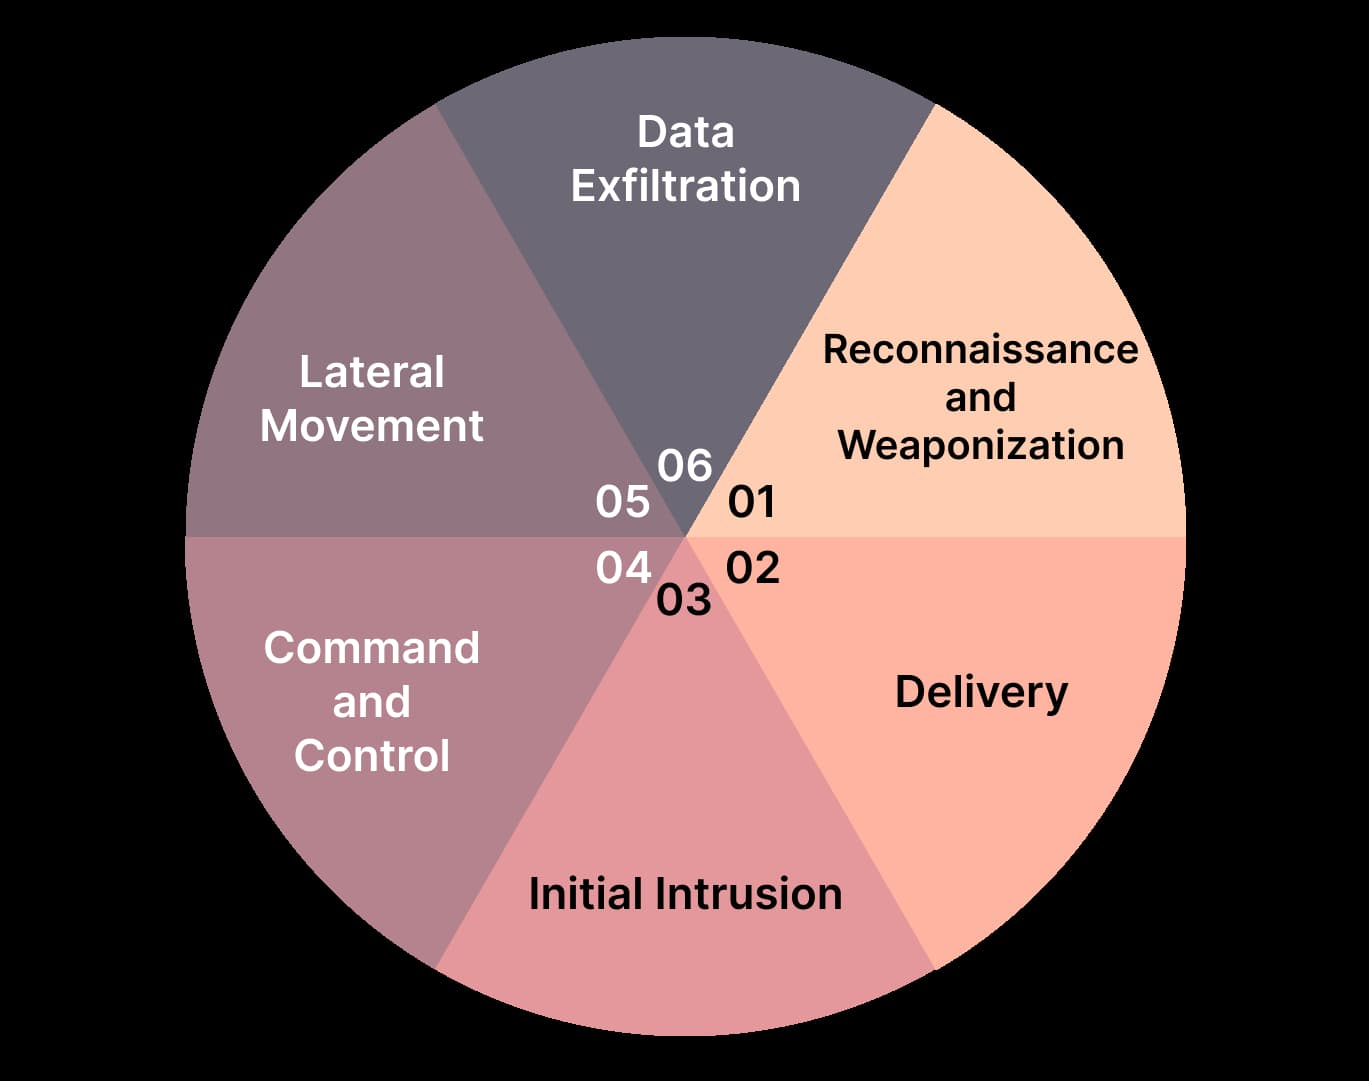
\includegraphics[width=0.8\textwidth]{src/images/chapter2/apt-lifecircle.jpg}
    \caption[Vòng đời của tấn công APT]{Vòng đời của tấn công APT \cite{chen2014apt}}
    \label{fig:apt-lifecircle}
\end{figure}

\bigbreak\noindent
Đã có các nghiên cứu nhằm đưa ra được một vòng đời hoạt động của tấn công APT một cách chính xác nhất. Trong khóa luận này, chúng tôi sử dụng vòng đời APT được đề xuất trong \cite{chen2014apt} như trong \textbf{Hình \ref{fig:apt-lifecircle}}. Cụ thể, vòng đời của một cuộc tấn công APT được đề xuất bao gồm sáu giai đoạn theo thứ tự như sau: \textit{trinh sát và vũ khí hoá}, \textit{vận chuyển}, \textit{bước đầu xâm nhập}, \textit{ra lệnh và kiểm soát}, \textit{lan rộng}, \textit{trích xuất thông tin}.

\begin{itemize}
    \item \textit{Trinh sát và vũ khí hoá}: Trong giai đoạn này, kẻ tấn công sẽ xác định và tìm hiểu về mục tiêu, từ đó thu thập càng nhiều thông tin về mục tiêu càng tốt, bao gồm thông tin hệ thống, công nghệ, những người nắm giữ vai trò quan trọng. Tiếp theo đó, kế hoạch tấn công sẽ được xây dựng cùng với những tài nguyên cần thiết cho việc tấn công như là các mã độc chuyên dụng, máy chủ và nhân lực.
    \item \textit{Vận chuyển}: Sau khi chuẩn bị, kẻ tấn công sẽ thực hiện xâm nhập vào hệ thống trực tiếp hoặc gián tiếp. Với các trực tiếp, những công cụ khai thác sẽ được gửi đến những người trong hệ thống bằng cách sử dụng các kỹ thuật như lừa đảo qua mạng hoặc là sử dụng các kỹ thuật xã hội. Đối với cách gián tiếp, kẻ tấn công sẽ âm thầm khai thác những bên thứ ba được mục tiêu tin cậy và từ đó xâm nhập vào hệ thống.
    \item \textit{Bước đầu xâm nhập}: Những công cụ đã được gửi vào hệ thống từ bước trước đó sẽ được kích hoạt và thực hiện tấn công lần đầu, thiết lập chỗ đứng của bản thân trong hệ thống và sau đó tạo các cổng giao tiếp bí mật ra bên ngoài.
    \item \textit{Ra lệnh và kiểm soát}: Sau khi có thể kết nối đến với máy nạn nhân, kẻ tấn công thực hiện nhiều cuộc khai thác có chủ đích vào trong hệ thống của nạn nhân. Kẻ tấn công thường lợi dụng những công cụ, dịch vụ có sẵn trong hệ thống hoặc các công cụ chính thống phổ biến nhằm đảm bảo không bị phát hiện và qua mặt các công cụ bảo mật cùng với các chuyên gia bảo mật.
    \item \textit{Mở rộng phạm vi}: Kẻ tấn công thực hiện di chuyển trong mạng để tăng khả năng kiểm soát của mình ra toàn mạng, từ đó thu thập được các thông tin có giá trị nhất. Đây là giai đoạn kéo dài khá lâu vì kẻ tấn công muốn tối ưu lượng thông tin mình có thể thu thập được, cùng với đó là phải giữ cho không bị phát hiện.
    \item  \textit{Trích xuất thông tin}: Đây là một bước quan trọng, các thông tin thu thập được sẽ được nén lại và mã hoá. Sau đó, các thông tin này sẽ được truyền dẫn qua các kênh bí mật đến máy chủ được xây dựng và kiểm soát bởi kẻ tấn công.
\end{itemize}

\subsection{Cách phòng chống}

Thật không may, các phương pháp phòng thủ truyền thống chẳng hạn như tường lửa, các phần mềm diệt virus trên các thiết bị là không đủ sức ngăn chặn tấn công APT. Chính vì vậy, các nhà nghiên cứu đang tích cực phát triển các giải pháp bảo mật hiện đại, trong số có việc sử dụng phương pháp săn tìm mối đe dọa. Nội dung chi tiết sẽ được chúng tôi trình bày tại \textbf{Mục \ref{Chapter2_ThreatHunting}}.

\section{Săn tìm mối đe dọa}\label{Chapter2_ThreatHunting}

\subsection{Tổng quan về săn tìm mối đe dọa}

Có rất nhiều phương pháp đã được nghiên cứu và sử dụng nhằm tăng khả năng bảo mật của hệ thống trước các mối đe dọa. Tuy nhiên, hầu hết chúng đều là các phương pháp giám sát, phát hiện các cuộc tấn công một cách bị động hoặc chờ đợi phản ứng lại. Đối với các cuộc tấn công kiểu mới, đặc biệt là tấn công APT, việc giám sát các dấu vết để lại là rất khó khăn vì khả năng che dấu hành vi của chúng. Chính vì thế, một phương pháp chủ động hơn như là săn tìm mối đe doạ cần được sử dụng.

\bigbreak\noindent
Săn tìm mối đe dọa là quá trình phân tích chủ động do các nhà săn tìm tiến hành để tìm kiếm các chiến thuật, kỹ thuật và thủ tục (TTP) của các mối đe dọa trong hệ thống nhằm đảm bảo ngăn chặn được các cuộc tấn công trước khi nó xảy ra, hoặc ít nhất sẽ phát hiện sớm các cuộc tấn công đang tồn tại trong hệ thống nhưng chưa bị phát hiện.

\subsection{Quy trình tiến hành}

Hình \ref{fig:threat-hunting-life-circle} biểu diễn quy trình tiến hành săn tìm mối đe doạ bao gồm sáu giai đoạn như sau: \textit{xác định mục đích}, \textit{xác định phạm vi săn tìm}, \textit{chuẩn bị}, \textit{xem xét kế hoạch}, \textit{săn tìm}, \textit{phản hồi}.

\begin{figure}[h]
    \centering
    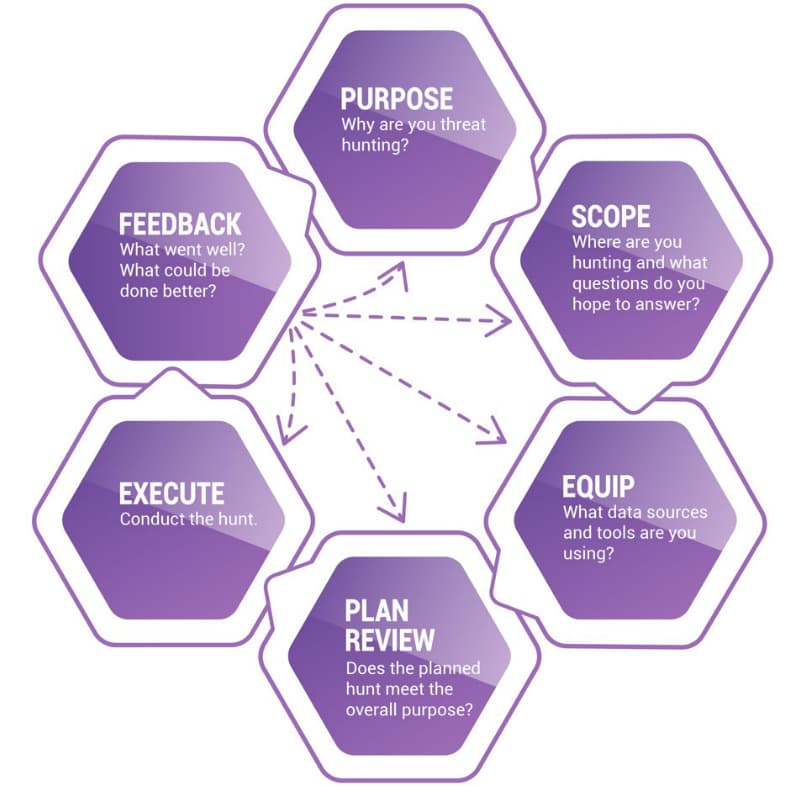
\includegraphics[width=0.8\textwidth]{src/images/chapter2/threat-hunting-life-circle.jpg}
    \caption[Quy trình tiến hành săn tìm mối đe dọa]{Quy trình tiến hành săn tìm mối đe dọa \cite{gunter2018practical}}
    \label{fig:threat-hunting-life-circle}
\end{figure}

\bigbreak\noindent
\textbf{Xác định mục đích}
\bigbreak\noindent
Giai đoạn đầu tiên là xác định mục tiêu của cuộc săn tìm, và được chọn dựa trên mục đích của tổ chức tiến hành săn tìm. Trong giai đoạn này, ba vấn đề sẽ được giải quyết nhằm tìm ra hướng đi, cụ thể như sau:

\begin{itemize}
    \item \textit{Mục đích của cuộc săn tìm?}: Lý do tại sao cần phải tiến hành săn tìm.
    \item \textit{Cuộc săn tìm sẽ được diễn ra trong phạm vi nào?}: Việc xác định mục tiêu cũng bao gồm phạm vi, môi trường tiến hành nhằm xác định các định và hạn chế của cuộc săn tìm.
    \item \textit{Kết quả mong muốn đạt được khi tiến hành cuộc săn tìm?}: Kết quả mong muốn phải phù hợp với các mục tiêu của tổ chức và cách tiến hành săn tìm mối đe dọa hỗ trợ giảm thiểu rủi ro ra sao.
\end{itemize}

\bigbreak\noindent
Một ví dụ cho việc tại sao cuộc săn tìm diễn ra như là khi một chức thực hiện triển khai một hệ thống mạng mới, việc tiến hành săn tìm giúp đảm bảo an toàn và tăng sự tự tin đối với hệ thống mạng mới. Việc xác định có thể tiến hành toàn bộ hoặc một phần mạng mới tuỳ vào chiến lược của tổ chức. Cuối cùng, mục tiêu mong muốn có thể là tìm ra được các lỗ hổng hay có những cuộc tấn công đã tồn tại trong hệ thống mạng mới. 

\bigbreak\noindent
\textbf{Xác định phạm vi săn tìm}
\bigbreak\noindent
Ở giai đoạn này, từ phạm vi đã được xác định ở giai đoạn \textit{xác định mục đích}, phạm vi sẽ được cụ thể hoá, như là việc xác định rõ một hệ thống hay một khu vực mạng tiến hành săn tìm. Bên cạnh đó, các giả thuyết phù hợp với lại mục tiêu của cuộc săn tìm sẽ được được đặt ra trong giai đoạn này. Trong giai đoạn \textit{xác định mục đích săn tìm}, có hai bước cần được hoàn thành tuần tự như sau: \textit{chọn ra các hệ thống được tiến hành săn tìm} và \textit{phát triển giả thuyết}.

\bigbreak\noindent
Tại bước \textit{chọn ra các hệ thống được tiến hành săn tìm}, ta có thể bắt đầu từ việc xác định các cơ sở cụ thể, hay có thể là các mạng hay mạng con. Tiếp theo đó, phạm vi được thu hẹp bằng cách lựa chọn các hệ thống quan trọng, đảm bảo hỗ trợ mục đích tổng thể của cuộc săn lùng. Các lỗi phổ biến bước này bao gồm việc đặt phạm vi của cuộc săn lùng quá hẹp dẫn đến bỏ qua sự hiện diện của kẻ tấn công trong môi trường.

\bigbreak\noindent
Tiếp theo, tại bước \textit{phát triển giả thuyết}, các giả thuyết sẽ được tạo ra cho cuộc săn tìm. Trong săn tìm mối đe dọa, giả thuyết là một đề xuất liên quan đến TTP của các mối đe dọa, thường bắt nguồn từ thông tin tình báo, cơ sở dữ liệu, nghiên cứu bảo mật, kinh nghiệm hoặc trực giác của chuyên gia, sau đó được cho là đúng hoặc tạm thời là đúng. Giả thuyết giữ vai trò duy trì sự tập trung của cuộc săn lùng và xác định hướng đi của cuộc săn lùng mối đe dọa. Một giả thuyết được định nghĩa bao gồm ba yếu tố:

\begin{itemize}
    \item \textit{Loại của giả thuyết}: Các giả thuyết có thể được phân thành ba loại, dựa trên thông tin tình báo, kiến thức và nhận thức về tình hình.
    \item \textit{Mục tiêu của giả thuyết}: Một giả thuyết thường chỉ nên tập trung vào một phần của hệ thống nhằm đảm bảo sự rõ ràng. Và nhiều giả thuyết sẽ được đặt ra nhằm đảm bảo cuộc săn tìm sẽ tập vào toàn bộ hệ thống đã được chọn.
    \item \textit{Xác định câu hỏi phân tích cần được trả lời}
\end{itemize}

\bigbreak\noindent
\textbf{Chuẩn bị}
\bigbreak\noindent
Giai đoạn \textit{chuẩn bị} tập trung vào việc phát triển một kế hoạch thu thập và phân tích dữ liệu toàn diện. Kế hoạch chuẩn bị bao gồm việc sử dụng các nguồn dữ liệu và chuẩn bị các TTP mà cuộc săn tìm sẽ sử dụng để trả lời các giả thuyết đã được phát triển. Giai đoạn này sẽ được tiến hành bao gồm hai bước: \textit{xác định nguồn dữ liệu} và \textit{xác định phương pháp phân tích}.

\bigbreak\noindent
Với bước \textit{xác định nguồn dữ liệu}, nguồn dữ liệu sẽ được chọn lọc từ các nguồn dữ liệu có tiềm năng, đánh giá xem chúng có giúp ích cho việc đưa ra quyết định chấp thuận hay bác bỏ giả thuyết hay không.

\bigbreak\noindent
\textbf{Xem xét kết hoạch}
\bigbreak\noindent
Giai đoạn \textit{xem xét kế hoạch} là một bước chạy đà để đảm bảo rằng kế hoạch săn tìm mối đe dọa đáp ứng các mục tiêu đã được đề ra. Giai đoạn này cũng bao gồm việc xác định các khuyết điểm và đề xuất các giải pháp tiềm năng, đồng thời phân bổ các tài nguyên bổ sung cần thiết để thực hiện cuộc săn tìm. Các tài nguyên bổ sung có thể bao gồm nhân lực, tài chính, kỹ thuật, hoặc tái thiết lại toàn bộ cuộc săn tìm. Cuối cùng, việc xem xét kế hoạch cũng nên đảm bảo xem xét thời gian mà cuộc săn lùng sẽ tiêu tốn và đảm bảo rằng khoảng thời gian cho cuộc săn lùng đủ cho việc thu thập dữ liệu.

\bigbreak\noindent
\textbf{Săn tìm}
\bigbreak\noindent
Sau khi kế hoạch săn lùng được phê duyệt, giai đoạn \textit{săn tìm} được tiến hành, bao gồm nhiều vòng lặp của việc thu thập và phân tích dữ liệu. Thông tin được thu thập như đã được xác định trong giai đoạn \textit{xác định phạm vi săn tìm} và sử dụng các kỹ thuật phân tích để chứng minh hoặc bác bỏ các giả thiết đã được phát triển. Các bộ dữ liệu khác có sẵn và các kỹ thuật phân tích không nằm trong cuộc săn tìm cũng nên được bổ sung khi cần thiết để đáp ứng mục đích của cuộc săn tìm.

\bigbreak\noindent
\textbf{Phản hồi}
\bigbreak\noindent
Giai đoạn \textit{phản hồi} cung cấp một cái nhìn tổng quan đối với tất cả các giai đoạn trước đó cũng như là tác động chi tiết của chúng đối với cuộc săn tìm. Các câu hỏi sẽ được đặt ra với mỗi giai đoạn. Dưới đây là các câu hỏi với các giai đoạn \textit{xác định phạm vi săn tìm}, \textit{chuẩn bị}, \textit{xem xét kế hoạch}, \textit{săn tìm}.

\bigbreak\noindent
Phản hồi đối với với giai đoạn \textit{xác định phạm vi săn tìm}, các câu hỏi có thể được đặt ra như: Mức độ hoàn thành của giai đoạn? Việc chọn giả thuyết có hiệu quả không? Các nguồn thông tin tình báo có hiệu quả cho việc chọn giả thuyết không? ... Bên cạnh đó, các câu trả lời cho những câu hỏi này nên góp phần vào việc tổ chức các cuộc săn lùng trong tương lai một cách hiệu quả hơn dựa trên những điểm mạnh và hạn chế từ các tổng kết trước đây.

\bigbreak\noindent
Phản hồi của giai đoạn chuẩn bị tập trung vào việc các tập dữ liệu và kỹ thuật phân tích có hỗ trợ tốt cho cuộc săn lùng hay không, từ đó đưa ra biện pháp cải thiện. Một số câu hỏi được đặt như: Các nguồn dữ liệu đã được xác định chưa? Những kỹ thuật phân tích  Liệu yêu cầu có phù hợp với kết quả dự kiến không? ... Ngoài ra, giai đoạn này cũng đề xuất các kỹ thuật phân tích tự động hoá với những phần có thể, và những phần còn lại có thể dùng các kỹ thuật thủ công.

\bigbreak\noindent
Phản hồi cho giai đoạn \textit{xem xét kế hoạch} đưa ra nhận định về mức độ giữ cho cuộc săn lùng tập trung vào mục đích. Các câu hỏi được đưa ra: Việc xem xét có phát hiện được bất kỳ vấn đề nào không? Có những câu hỏi nào khác nên được tích hợp vào giai đoạn \textit{xem xét kế hoạch} không? ... Ngoài ra, có thể phản hồi về việc phân bổ tài nguyên cho cuộc săn tìm hợp lý hay không.

\bigbreak\noindent
Giai đoạn \textit{săn tìm} sẽ được phản hồi về việc thu thập dữ liệu, phân tích và thay đổi dữ liệu. Những câu hỏi có thể sử dụng như: Có sử dụng đúng công cụ và kỹ thuật không? Những yếu tố nào ảnh hưởng đến cuộc săn tìm? ...  Thêm vào đó, ta cũng có thể đánh giá hiệu suất của việc sử dụng các kỹ thuật phân tích đối với các nguồn dữ liệu nhằm phát hiện các dấu hiệu liên quan đến sự hiện diện của kẻ tấn công.

\subsection{Các vấn đề liên quan đến săn tìm mối đe dọa}\label{chapter2_th_problems}

\bigbreak\noindent
\textbf{Các trở ngại cho việc áp dụng săn tìm mối đe dọa}
\bigbreak\noindent
Hiện tại, theo một cuộc khảo sát bởi SANS năm 2022\footnote{SANS Threat hunting suvey 2022: \url{https://www.sans.org/white-papers/sans-2022-threat-hunting-survey/}} thì vấn đề về con người và công nghệ là những trở ngại lớn nhất được biểu diễn tại \textbf{Hình \ref{fig:threat-hunting-barriers}}. Vấn đề nan giải nhất được xem là con người. Khi mà nguồn nhân lực chất lượng không đủ thì khó có thể tiến hành được việc săn tìm.

\bigbreak\noindent
Thiếu hụt công cụ và công nghệ cũng đang là lý do khiến nhiều tổ chức không thể tổ chức săn tìm. Mặc dù không thể thay thế được con người, tuy nhiên, việc có được sự hỗ trợ của các công cụ và công nghệ có thể một phần nào khỏa lấp vấn đề con người trong săn tìm mối đe hoạ. Đây là vấn đề đang nhận được sự quan tâm và nghiên cứu, một số nghiên cứu đã được đề cập tại Chương \ref{Chapter1} như \cite{jadidi2021threat}, \cite{caltagirone2013diamond}, \cite{ajmal2021offensive}, ... Và trong đề tài này, chúng tôi cũng muốn đưa ra một giải pháp nhằm có thể giải quyết một phần nào vấn đề thiếu hụt công nghệ này.

\begin{figure}[h]
    \centering
    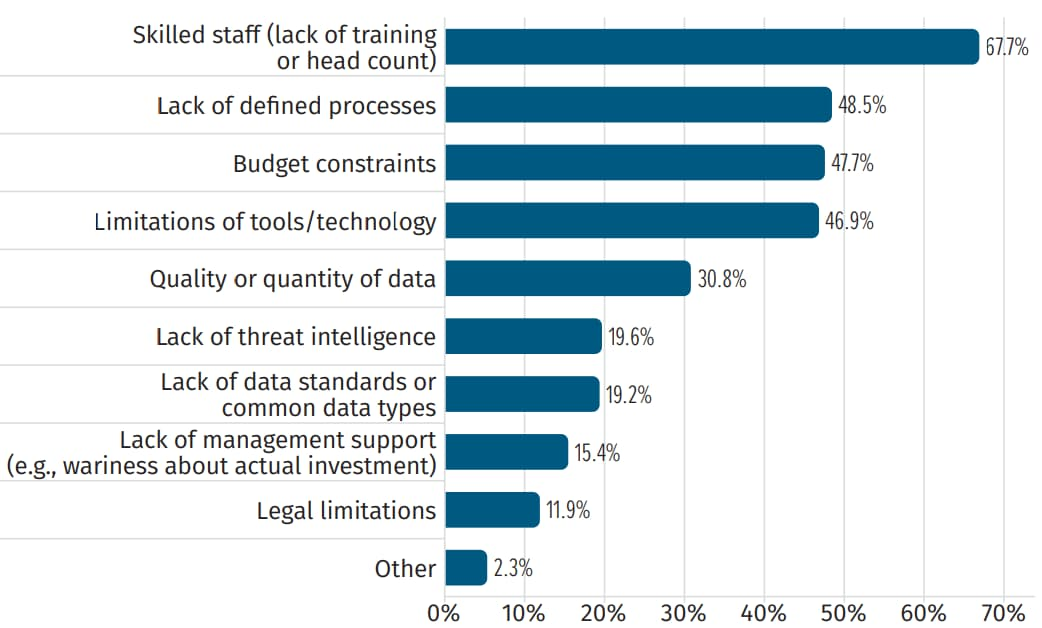
\includegraphics[width=\textwidth]{src/images/chapter2/threat-hunting-barriers.jpg}
    \caption[Các trở ngại cho việc áp dụng săn tìm mối đe dọa]{Các trở ngại cho việc áp dụng săn tìm mối đe dọa, theo cuộc khảo sát từ SANS 2022}
    \label{fig:threat-hunting-barriers}
\end{figure}

\bigbreak\noindent
\textbf{Những công nghệ được áp dụng trong săn tìm mối đe dọa}
\bigbreak\noindent
Cũng theo cuộc khảo sát của SANS năm 2022, các giải pháp như SIEM và IDS có được sự tăng trưởng vượt trội về mức độ sử dụng được thể hiện tại \textbf{Hình \ref{fig:threat-hunting-technologies}}, và các nền tảng cung cấp CTI cũng có được mức độ sử dụng cao. Những công nghệ này đã được áp dụng vào nhiều tổ chức và có mức độ tin cậy cao cho săn tìm mối đe dọa. Bên cạnh đó, tuy không có được mức độ sử dụng như các giải pháp kể trên, trí tuệ nhân tạo đang bắt đầu được tin tưởng và sử dụng vào trong săn tìm mối đe dọa. Chúng tôi nhận thấy đây là các công nghệ tiềm năng, có thể phát triển và nghiên cứu nhằm cung cấp một mô hình săn tìm mối đe dọa có hiệu năng cao và ổn định.

\begin{figure}[h]
    \centering
    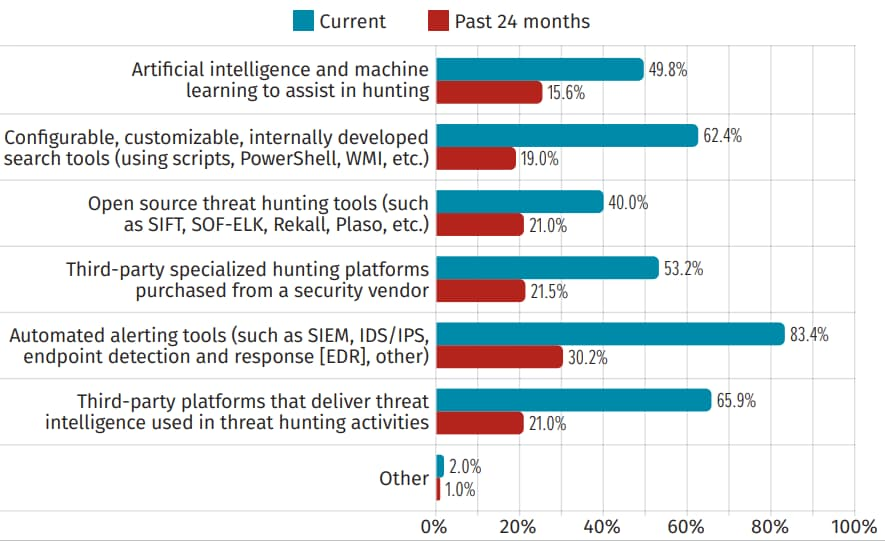
\includegraphics[width=\textwidth]{src/images/chapter2/threat-hunting-technologies.jpg}
    \caption[Tỉ lệ của những công nghệ được sử dụng vào săn tìm mối đe dọa]{Tỉ lệ của những công nghệ được sử dụng vào săn tìm mối đe dọa năm 2022 được biểu thị bằng xanh dương và vào 24 tháng trước được biểu thị bằng màu đỏ}
    \label{fig:threat-hunting-technologies}
\end{figure}

\section{Hệ thống IDS}\label{Chapter2_IDS}

\subsection{Tổng quan}

IDS là một thiết bị phần cứng hoặc là phần mềm được sử dụng nhằm giám sát các hoạt động bất thường và các hành động trái với chính sách của hệ thống mạng. IDS có thể thực hiện theo dõi hệ thống mạng trên nhiều phạm vi khác nhau, từ các máy tính đơn lẻ cho đến những hệ thống mạng lớn.

\bigbreak\noindent
IDS phát hiện các mối đe dọa mạng và cảnh báo cho các quản trị viên bảo mật về mối đe dọa đã biết hoặc tiềm năng. Ngoài ra, các cảnh báo cũng có thể được gửi đến hệ thống an ninh tập trung như SIEM nhằm kết hợp dữ liệu từ các nguồn khác với cảnh báo được đưa ra, từ đó xác định và đáp ứng mối đe dọa khác nhau.

\subsection{Phân loại}

IDS có thể được phân loại theo nhiều cách khác nhau, như phân loại theo phạm vi mà IDS hoạt động hay cách mà IDS sử dụng nhằm phát hiện tấn công. Dưới đây hai loại IDS được phân loại theo cách thức phát hiện:

\begin{itemize}
    \item \textit{IDS dựa trên đặc điểm (Signature-based IDS)}: Phát hiện dựa trên việc so sánh với những mẫu tấn công đã biết trước trong cơ sở dữ liệu. Đối với những cuộc tấn công đã được đưa vào cơ sở dữ liệu , CÁc hệ thống IDS dạng này có kết quả dự đoán chính xác cao. Tuy nhiên, để đảm bảo được độ chính xác cao, cơ sở dữ liệu cho hệ thống IDS dựa trên đặc điểm phải được được cập nhật thường xuyên. Tuy nhiên, trước sự phát triển của các cuộc tấn công kiểu mới như là tấn công APT thì việc đảm bảo cơ sở dữ liệu có tồn tại hay cập nhật được được mẫu tấn công của chúng là rất khó khăn, dẫn đến sự thiếu hiệu quả của các hệ thống IDS sử dụng mô hình này.
    \item \textit{IDS dựa trên bất thường (Anomaly-based IDS)}: IDS dựa trên bất thường nhận được rất nhiều sự quan tâm vì nó thể vượt qua những hạn chế của IDS dựa trên đặc điểm. Các hệ thống IDS dạng này có thể phát hiện các cuộc tấn công kiểu mới nhờ vào khả năng phát hiện phát hiện không phụ thuộc vào đặc điểm. Nó phát hiện những cuộc tấn công bằng cách tìm ra những hành vi khác thường so với những hành vi bình thường trong hệ thống. Các mẫu hành vi bình thường được tạo ra bằng cách dựa trên dữ liệu có được, thống kê, hoặc cả trí tuệ nhân tạo. Dù hiệu quả là vậy, IDS dựa trên bất thường cũng gặp phải một số vấn đề như báo động giả và về hiệu năng.
\end{itemize}

\bigbreak\noindent
Dựa trên phạm vi theo dõi, IDS bao gồm hai loại:

\begin{itemize}
    \item \textit{NIDS}: Các lưu lượng mạng ra vào toàn mạng được quản lý và giám sát, cung cấp cái nhìn toàn cảnh về những cuộc tấn công nhiều mục tiêu trong mạng. Tuy nhiên việc theo dõi từng thành phần trong mạng lại không được chi tiết và chính xác.
    \item \textit{HIDS}: Thực hiện giám sát các thành phần chỉ định trong mạng chẳng hạn như máy tính các nhân, máy chủ, ... Việc giám sát riêng biệt giúp đảm bảo an toàn một cách tối ưu hơn cho thành phần chỉ định. Mặc dù vậy, HIDS cũng có những hạn chế nhất định như tiêu tốn tài nguyên của thành phần được giám sát, phạm vi giám sát hẹp
\end{itemize}

\bigbreak\noindent
Các loại IDS đều có ưu và nhược điểm, việc sử dụng riêng lẻ hoặc kết hợp nhiều loại IDS tuỳ thuộc vào ngữ cảnh của hệ thống mạng sao cho có thể đạt được hiệu năng theo dõi cũng như tính bảo mật cao nhất.

\subsection{Tính cấp thiết trong việc cải thiện IDS}

IDS vẫn luôn là một giải pháp bảo mật tin cậy và được sử dụng rộng rãi bởi các tổ chức. Nó cũng là một công nghệ được sử dụng phổ biến trong săn tìm mối đe doạ nhằm tìm ra các cuộc tấn công kiểu mới, như tấn công APT, theo như đã đề cập tại \textbf{Mục \ref{chapter2_th_problems}}. Dù vậy, bản thân IDS thì khó có thể phát hiện được các cuộc tấn công ngày càng tinh vi và phức tạp, với khả năng trốn tránh và qua mặt các hệ thống bảo mật một cách dễ dàng.

\bigbreak\noindent
Nhận thấy được vấn đề này, nhiều nghiên cứu đã đề xuất các giải pháp IDS kiểu mới, có thể kể đến như \cite{yazdinejadna2021kangaroo}, \cite{chen2022building}, \cite{lo2022graphsage}, ... Tuy nhiên, chúng tôi cũng nhận thấy rằng, IDS vẫn cần được nghiên cứu và cải thiện hơn nữa. Trong đề tài này, chúng tôi cũng đưa ra một giải pháp IDS nhằm phát hiện các cuộc tấn công APT một cách hiệu quả, từ đó cung cấp một giải pháp săn tìm mối đe dọa ổn định.

% Ngoài hai cách phát hiện trên, đã có nhiều nghiên cứu tích hợp IDS với các phương pháp phát hiện khác nhau. Trong đề tài này, chúng tôi có sử dụng thêm một loại IDS là IDS dựa trên việc truy vết (PIDS). PIDS sử dụng các dữ liệu truy vết, cụ thể như đồ thị nguồn gốc nhằm tìm kiếm các bất thường trong hệ thống dựa vào các hành động, thời gian, các mối quan hệ giữa các sự kiện trong hệ thống. Chi tiết về đồ thị nguồn gốc sẽ được chúng tôi trình bày tại \textbf{Mục \ref{Chapter2_PG}}.

\section{Đồ thị nguồn gốc}\label{Chapter2_PG}

\subsection{Tổng quan}

Đồ thị nguồn gốc là một loại đồ thị dữ liệu và phương pháp phân tích được sử dụng để theo dõi và ghi lại nguồn gốc, lịch sử và quá trình xử lý của dữ liệu trong một hệ thống an toàn thông tin như trong \textbf{Hình \ref{fig:provenance-graph}}. Nó được xem như một công cụ quan trọng để phát hiện và phân tích các hoạt động độc hại, xâm nhập hoặc thay đổi không mong muốn trong hệ thống. Đồ thị nguồn gốc, cũng như các đồ thị thông thường, bao gồm các nút và cạnh. Nút biểu diễn các thực thể trong hệ thống như tập tin, thư mục, tiến trình, gói tin mạng, và các đối tượng có tương tác với hệ thống. Cạnh biểu diễn mối liên hệ giữa các nút, như là các sự kiện, hành động tương tác. Với mỗi nút và cạnh, chúng có thể có các thuộc tính như các thông tin ngữ cảnh, thông tin thuộc tính với mỗi loại nút và cạnh.

\begin{figure}[h]
    \centering
    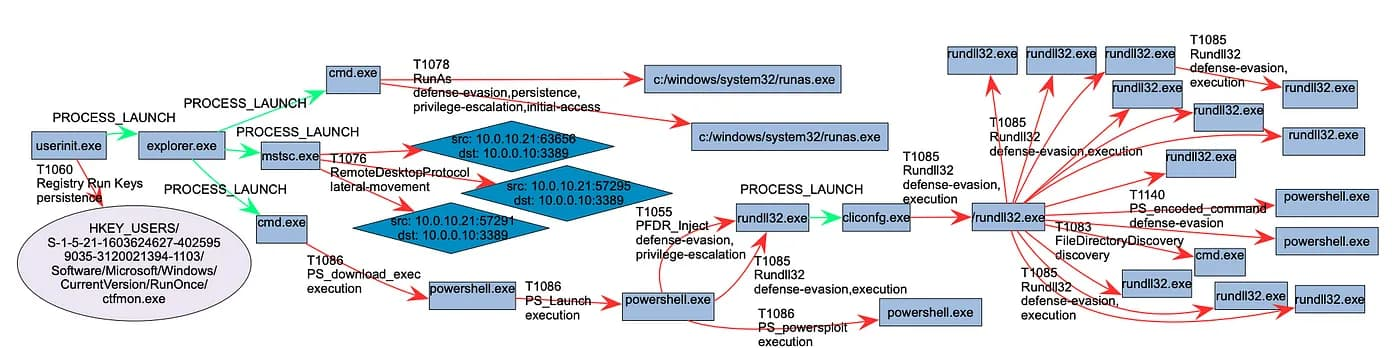
\includegraphics[width=\textwidth]{src/images/chapter2/provenance-graph.jpg}
    \caption{Ví dụ về đồ thị nguồn gốc}
    \label{fig:provenance-graph}
\end{figure}

\bigbreak\noindent
Đồ thị nguồn gốc cho phép chúng ta theo dõi lịch sử và nguồn gốc của các thực thể, sự kiện xảy ra trong hệ thống, cung cấp khả năng phát hiện và phân tích các hoạt động độc hại, xâm nhập hoặc thay đổi không mong muốn trong hệ thống. Bằng cách phân tích cấu trúc và mối quan hệ trong đồ thị nguồn gốc, chuyên gia an toàn thông tin có thể xác định các dấu hiệu và mối quan hệ giữa các thành phần trong hệ thống. Điều này cung cấp cơ sở cho việc đánh giá và đề xuất biện pháp phòng ngừa nhằm giảm thiểu các mối đe dọa an ninh và tăng cường bảo mật trong hệ thống.

\subsection{Tiềm năng đối với việc phát hiện tấn công APT}

Mặc dù tấn công APT áp dụng nhiều kỹ thuật trốn tránh tân tiến có thể qua mặt được nhiều hệ thống bảo mật, chúng vẫn có thể để lại dấu vết như các tương tác với môi trường trong hệ thống, các máy chủ bên ngoài, ... Với khả năng theo dõi về nguồn gốc trong hệ thống như đã đề cập ở trên, đồ thị nguồn gốc mang đến khả năng phát hiện các tấn công APT một cách hiệu quả. Đã có rất nhiều nghiên cứu về vấn đề này và chứng minh được sự hiệu quả. Cụ thể \cite{9739913} đã giới thiệu Paradise, một hệ thống phát hiện xâm nhập phân tán, tổng quát và thời gian thực, tận dụng các đặc điểm của đồ thị nguồn gốc nhằm phát hiện các cuộc tấn công. Còn với \cite{wei2021deephunter}, như đã đề cập tại \textbf{Mục \ref{chapter1:rel-works:xai-ids}}, các tác giả đã sử dụng việc so sánh đồ thị nguồn gốc và đồ thị hành vi tấn công APT đã biết ứng dụng GNN nhằm phát hiện các cuộc tấn công APT một các hiệu quả.

\section{Học sâu}

Học sâu là một phân nhánh của học máy sử dụng lượng dữ liệu lớn và thuật toán phức tạp để huấn luyện các mạng nơ-ron nhân tạo nhằm có thể thực hiện các nhiệm vụ phức tạp. Học sâu đã mang lại nhiều tiến bộ đáng kể trong công nghiệp, nghiên cứu và các lĩnh vực khác nhau với khả năng xử lý dữ liệu phức tạp và tạo ra những kết quả ấn tượng.

\subsection{Mạng nơ-ron nhân tạo}

Các mạng nơ-ron nhân tạo được lấy cảm hứng từ cách thức hoạt động của hệ thống thần kinh trong não người. Một mạng nơ-ron nhân tạo, như trong \textbf{Hình \ref{fig:neural-network}}, được xây dựng dựa trên các nơ-ron nhân tạo có khả năng tính toán. Các nơ-ron này được tổ chức thành nhiều lớp, bao gồm lớp đầu vào, các lớp ẩn và lớp đầu ra. Mỗi nút trong mạng nhận đầu vào từ các nút của lớp trước và tính toán đầu ra dựa trên các trọng số và hàm kích hoạt.

\begin{figure}[h]
    \centering
    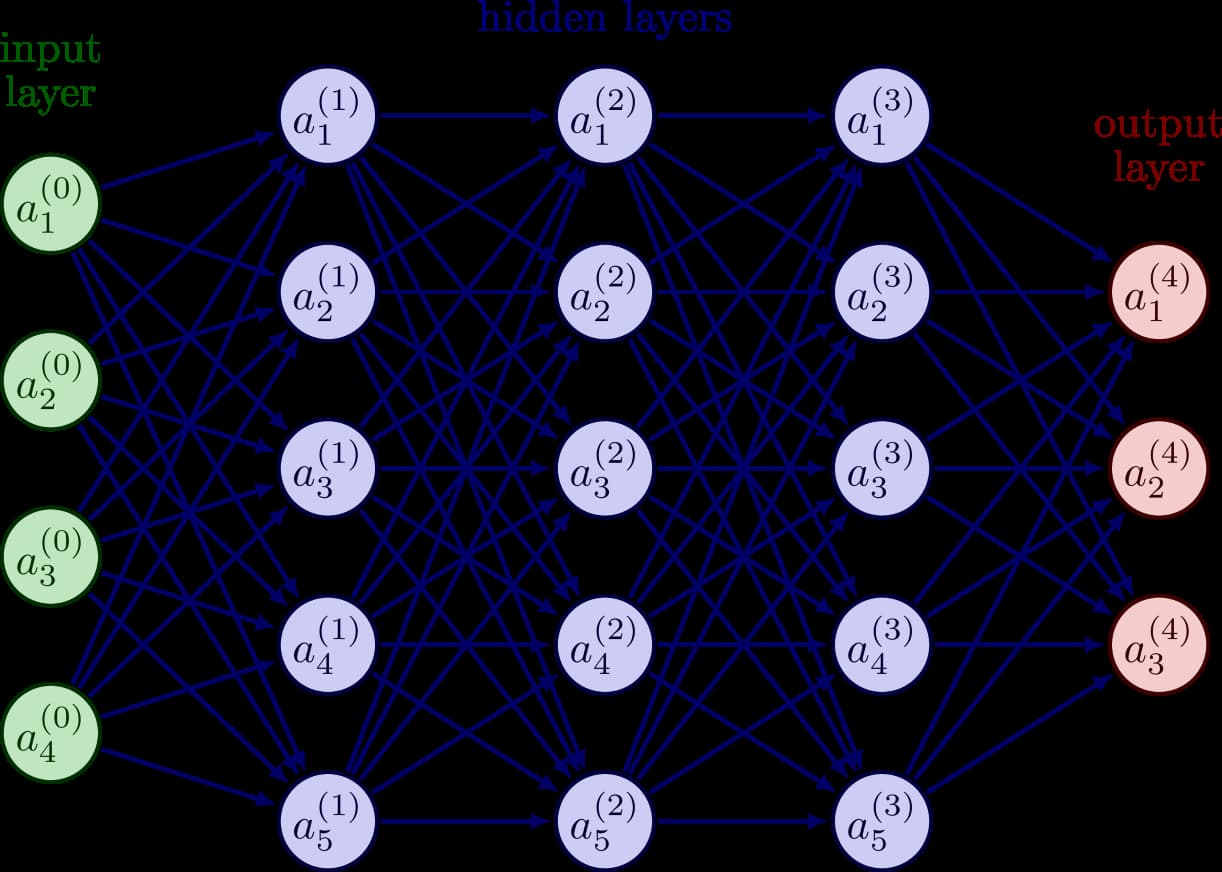
\includegraphics[width=\textwidth]{src/images/chapter2/neural-network.jpg}
    \caption{Ví dụ về mạng nơ-ron nhân tạo}
    \label{fig:neural-network}
\end{figure}

\bigbreak\noindent
Các trọng số trong mạng nơ-ron nhân tạo đóng vai trò quan trọng trong việc biểu diễn sự tương quan giữa các nơ-ron. Chúng biểu diễn tầm quan trọng của thông tin từ mỗi nơ-ron đầu vào và ảnh hưởng của nó đến đầu ra của nơ-ron tiếp theo. Quá trình điều chỉnh và tối ưu hóa các trọng số này là yếu tố quan trọng trong quá trình huấn luyện của mạng nơ-ron nhân tạo. Mục tiêu là điều chỉnh các trọng số sao cho hàm mất mát đạt được giá trị nhỏ nhất, tức là đầu ra dự đoán gần nhất với đầu ra thực tế.

\bigbreak\noindent
Để thực hiện quá trình tối ưu hoá, ta có thể sử dụng nhiều các khác nhau. Một trong những cách phổ biến nhất là sử dụng đạo hàm cho hàm mất mát. Khi giá trị đạo hàm dương, điều này chỉ ra rằng chúng ta đang di chuyển theo hướng tăng của hàm mất mát. Tuy nhiên, mục tiêu của chúng ta là tìm giá trị nhỏ nhất của hàm mất mát, do đó chúng ta cần thay đổi các trọng số sao cho đạo hàm di chuyển theo hướng giảm. Tại đây, hệ số \textit{tốc độ học (learning rate)} được sử dụng nhằm điều chỉnh tốc độ di chuyển của đạo hàm. Quá trình này tiếp tục cho đến khi đạt được điều kiện dừng, ví dụ như đạt được số lượng vòng lặp tối đa hoặc hàm mất mát không thay đổi đáng kể.

\bigbreak\noindent
Hàm kích hoạt là một thành phần quan trọng trong mạng nơ-ron nhân tạo và nó đóng vai trò quyết định trong việc xác định đầu ra của mỗi nơ-ron dựa trên đầu vào của nó. Hàm kích hoạt giúp đầu ra mang tính phi tuyến tính từ đầu vào tuyến tính của nơ-ron, cho phép mạng nơ-ron nhân tạo mô phỏng được các quan hệ phi tuyến trong dữ liệu sau đây là một số hàm kích hoạt:

\begin{itemize}
    \item \textit{Sigmoid}: Đưa ra đầu ra nằm trong khoảng từ 0 đến 1
    \begin{equation}
        \sigma(x) = \frac{1}{{1 + e^{-x}}}
    \end{equation}

    \item \textit{Softmax}: Đưa ra xác suất dự đoán cho mỗi lớp với bài toán phân loại nhiều lớp
    \begin{equation}
        \text{softmax}(x_i) = \frac{e^{x_i}}{\sum_{j=1}^{N} e^{x_j}}
    \end{equation}

    \item \textit{Tanh}: Đưa ra đầu ra nằm trong khoảng từ -1 đến 1
    \begin{equation}
        \tanh(x) = \frac{{e^x - e^{-x}}}{{e^x + e^{-x}}}
    \end{equation}

    \item \textit{ReLU}: Đưa ra đầu ra là các giá trị không âm
    \begin{equation}
        \text{ReLU}(x) = \max(0, x)
    \end{equation}
\end{itemize}

\subsection{Mạng CNN}

Mạng CNN là một kiến trúc mạng nơ-ron nhân tạo được thiết kế đặc biệt để xử lý và phân tích dữ liệu dạng lưới như hình ảnh. CNN đã đạt được thành công rực rỡ trong nhiều ứng dụng thị giác máy tính như nhận dạng vật thể, phân loại hình ảnh, nhận dạng khuôn mặt và xử lý ngôn ngữ tự nhiên. 

\begin{figure}[h]
    \centering
    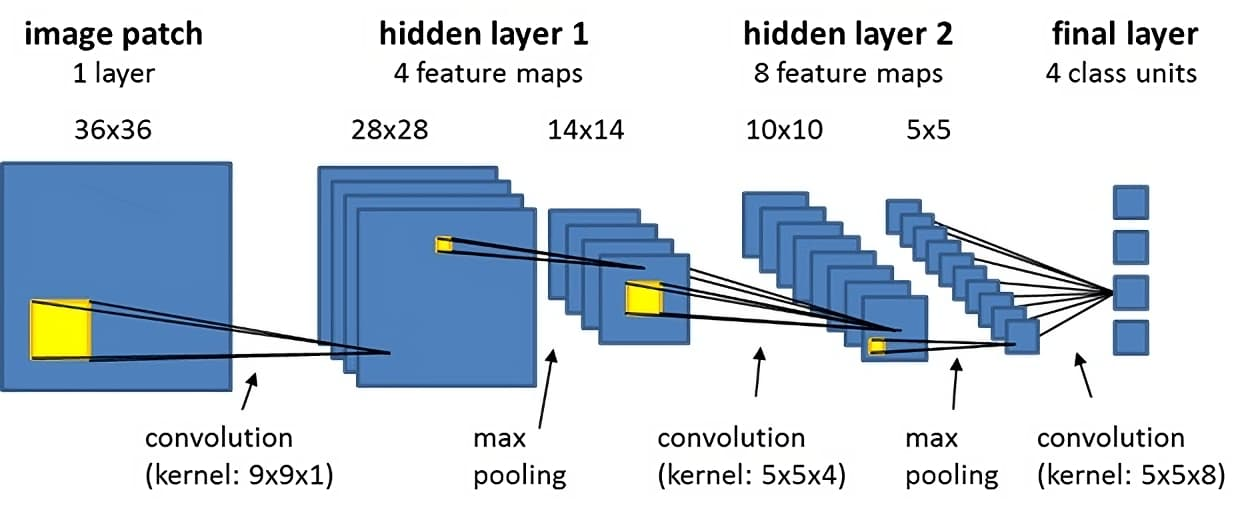
\includegraphics[width=\textwidth]{src/images/chapter2/cnn.jpg}
    \caption{Ví dụ về mạng CNN}
    \label{fig:cnn}
\end{figure}

\bigbreak\noindent
Mạng CNN thường được cấu tạo từ ba lớp chính: Lớp tích chập (convolutional layer), lớp tổng hợp (pooling layer) và lớp kết nối đầy đủ (fully connected layer).

% Mạng CNN thực hiện việc học các bộ lọc (kernel) tự động từ dữ liệu đầu vào. Những bộ lọc này được áp dụng thông qua các lớp tích chập (convolutional layers), với mỗi bộ lọc là một ma trận trọng số có kích thước nhỏ, và nó sẽ trượt qua các vùng tương ứng của dữ liệu đầu vào để tính toán tích chập và tạo ra các bản đồ thuộc tính (feature maps). Bên cạnh đó, các lớp gộp (pooling layers) thường được sử dụng để giảm kích thước của các bản đồ thuộc tính và tạo ra các bản đồ thuộc tính tổng hợp (pooled feature maps). Bản đồ thuộc tính thể hiện các thuộc tính ví dụ như cạnh, góc, hoặc các thuộc tính hình học khác, và biểu diễn thông tin về sự xuất hiện của những thuộc tính này trong dữ liệu.

\bigbreak\noindent
\textbf{Lớp tích chập}

\bigbreak\noindent
Lớp tích chập là thành phần chính, nắm giữ vai trò tính toán chính của mạng CNN. Lớp tích chập sử dụng các bộ lọc (kernel, filter), với mỗi bộ lọc là một tập hợp các tham số có thể học được với kích thước nhỏ. Tính toán tích chập được áp dụng trên các vùng cục bộ của dữ liệu đầu vào, cụ thể như sau: Bộ lọc sẽ thực hiện ``trượt" qua toàn bộ dữ liệu đầu vào theo một bước nhảy cố định (stride), là số lượng cột và hàng mà bộ lọc di chuyển trong một lần trượt. Sau đó phép tích vô hướng giữa bộ lọc và vùng cục bộ đang xét của dữ liệu đầu vào sẽ được thực hiện. Với mỗi kết quả tích vô hướng được xem là một điểm trong bảng đồ thuộc tính (feature map, activation map). Hình \ref{fig:cnn-convolutional-layer} minh hoạ về tính toán tích chập của lớp tích chập.

\begin{figure}[h]
    \centering
    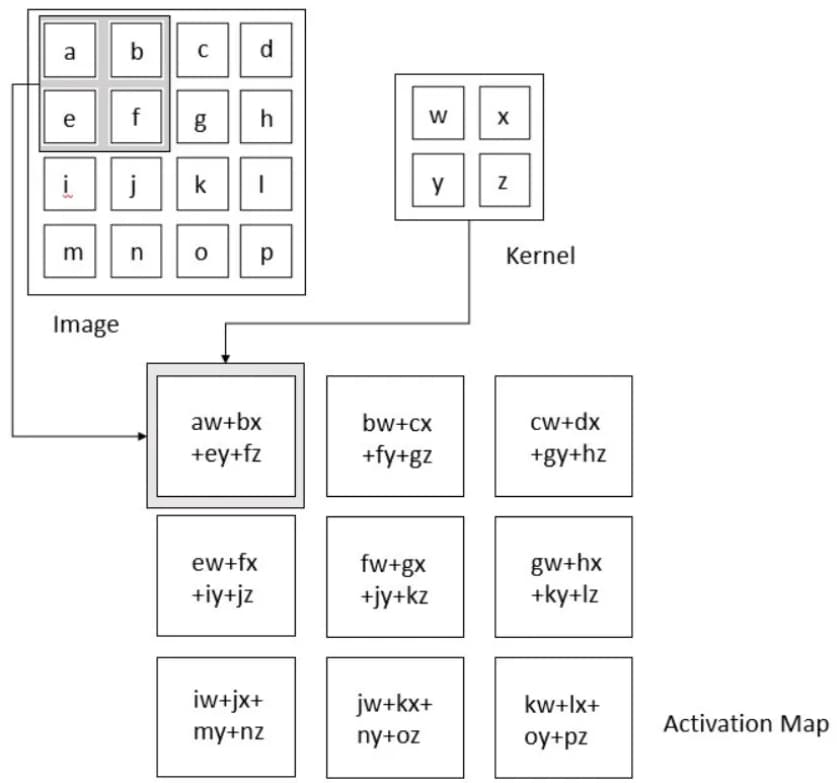
\includegraphics[width=0.6\textwidth]{src/images/chapter2/cnn-convolutional-layer.jpg}
    \caption[Ví dụ về tính toán tích chập trong của lớp tích chập trong mạng CNN]{Ví dụ về tính toán tích chập trong của lớp tích chập trong mạng CNN, với kích thước bộ lọc là 2x2 và kích thước bước nhảy là 1}
    \label{fig:cnn-convolutional-layer}
\end{figure}

\bigbreak\noindent
\textbf{Lớp tổng hợp}
Lớp tổng hợp là thực nghiệm việc giảm kích thước của dữ liệu đầu vào (thường là các bảng đồ thuộc tính) bằng cách lấy mẫu từ các vùng không gian lân cận và thực hiện một phép tổng hợp thông tin. Hình \ref{fig:cnn-pooling-layer} mô tả cách tổng hợp thông tin.

\begin{figure}[h]
    \centering
    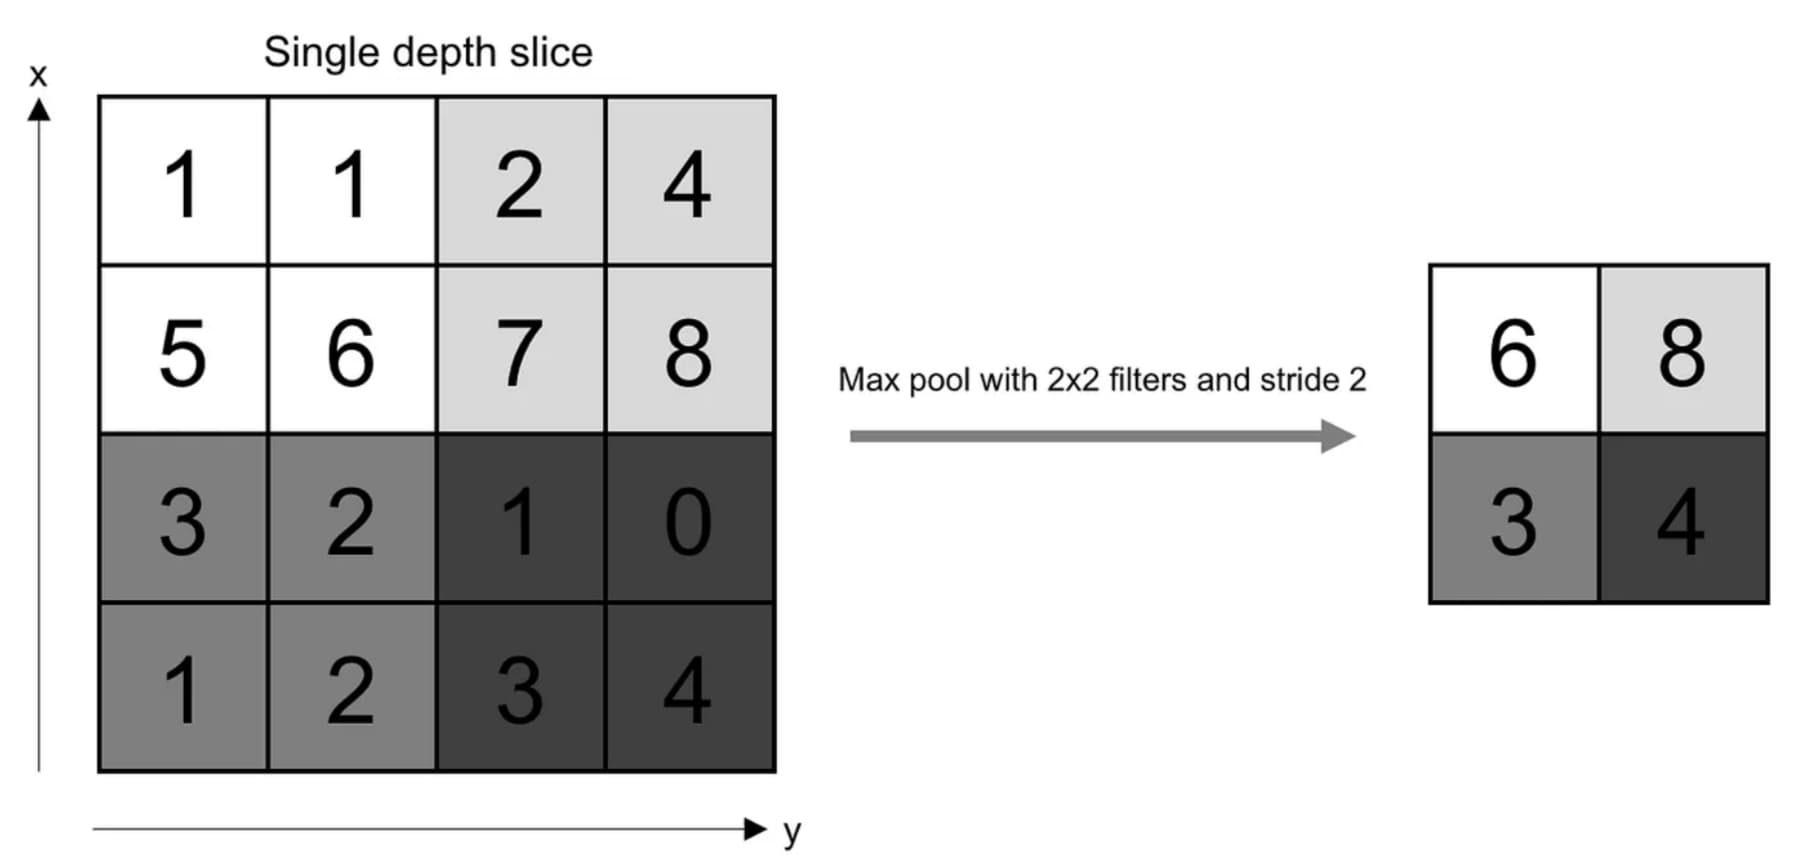
\includegraphics[width=\textwidth]{src/images/chapter2/cnn-pooling-layer.jpg}
    \caption{Ví dụ về tổng hợp thông tin của lớp tổng hợp}
    \label{fig:cnn-pooling-layer}
\end{figure}

\bigbreak\noindent
Có hai loại lớp tổng hợp thường được sử dụng:

\begin{itemize}
    \item \textit{Max pooling}: Chia dữ liệu đầu vào thành các vùng không trùng nhau và chọn giá trị lớn nhất từ mỗi vùng làm giá trị đại diện. Hình \ref{fig:cnn-pooling-layer} biểu diễn max pooling.
    \item \textit{Average pooling}: Tương tự như max pooling, tuy nhiên average pooling tính giá trị trung bình của các giá trị trong vùng làm giá trị đại diện.
\end{itemize}

\bigbreak\noindent
\textbf{Lớp kết nối đầy đủ}
Đầu ra của lớp tích chập là tuyến tính và dữ liệu đầu như là ảnh không phải là tuyến tính. Do đó, các lớp kết nối phi tuyến tính thường được đặt ngay sau lớp tích chập để biến đổi tính phi tuyến của bản đồ thuộc tính.

\subsection{Mạng GRU}

Mạng GRU là một loại kiến trúc mạng nơ-ron nhân tạo, là một phân nhánh mạng RNN. Trong các mạng RNN truyền thống, khi thông tin từ quá khứ truyền qua các lớp mạng, nó có thể bị mất dần qua thời gian và không đủ để đưa ra dự đoán chính xác. Nguyên nhân chính của vấn đề này là hiện tượng giảm gradient (Vanishing Gradient Problem) và vấn đề phụ thuộc dài hạn (Long-term Dependency problem). Mạng GRU được thiết kế để giải quyết vấn đề này bằng cách sử dụng các cổng để kiểm soát việc truyền thông tin trong quá trình lan truyền ngược.

\begin{figure}[h]
    \centering
    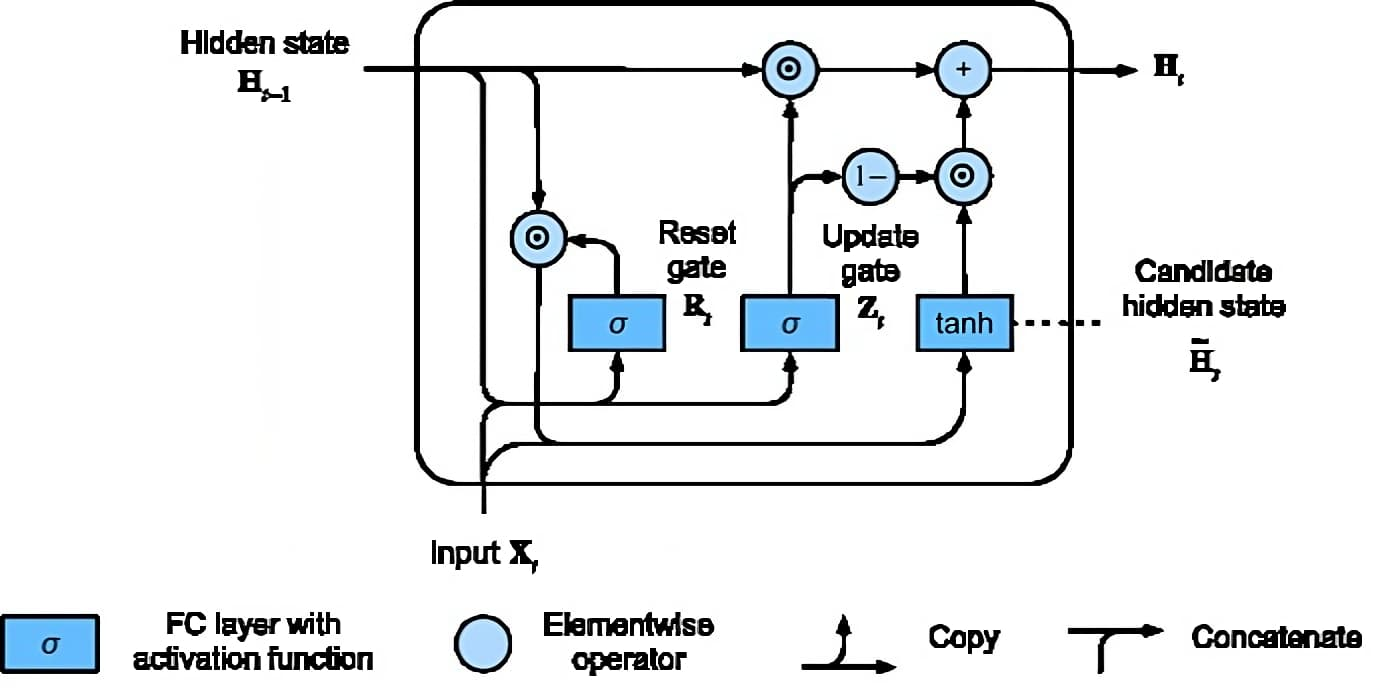
\includegraphics[width=\textwidth]{src/images/chapter2/gru.jpg}
    \caption{Kiến trúc của một đơn vị trong mạng GRU}
    \label{fig:GRU}
\end{figure}

\bigbreak\noindent
Mạng GRU được cấu tạo với nhiều đơn vị liên kết với nhau, với mỗi đơn vị có cấu tạo như sau:

\begin{itemize}
    \item \textit{Cổng cập nhật (Update Gate)}: Cổng này quyết định thông tin nào từ đầu vào hiện tại và trạng thái trước đó sẽ được cập nhật và chuyển tiếp tới các bước tiếp theo của mạng.
    \item \textit{Cổng quên (Reset Gate)}: Cổng này quyết định thông tin nào đơn vị trước sẽ được ``quên" và không được chuyển tiếp tới các đơn vị tiếp theo của mạng.
    \item \textit{Trạng thái ẩn (Hidden State)}: Đây là trạng thái hiện tại của mạng, chứa thông tin được tích lũy từ các bước trước đó và được cập nhật dựa trên cổng cập nhật và cổng quên.
    \item \textit{Đầu ra (Output):} Đầu ra của mạng GRU, có thể được lấy từ trạng thái ẩn hoặc có thể là một phần của trạng thái ẩn.
\end{itemize}


\subsection{Mạng GNN}

\textbf{Đồ thị}

\bigbreak\noindent
Đồ thị chính là thành phần cơ bản nhất của mạng GNN. Đồ thị là một dạng cấu trúc dữ liệu bao gồm các nút (nodes, vertices) và các cạnh (edges). Mỗi nút trong đồ thị đại diện cho một đối tượng, trong khi các cạnh đại diện cho các mối quan hệ hoặc kết nối giữa các đối tượng đó. Trên một đồ thị, mỗi nút có thể có các thuộc tính hoặc thuộc tính riêng, và các cạnh có thể có các thuộc tính hoặc trọng số. Sự kết hợp của các nút và cạnh tạo ra một biểu diễn phức tạp của mạng lưới các mối quan hệ trong hệ thống. Một số ví dụ cho đồ thị như là các phân tử hoá học, các mối quan hệ xã hội, các trích dẫn giữa các bài báo, ... và cả các dạng đồ thị không ngờ tới như hình ảnh, văn bản, ...

\begin{figure}[ht]
    \centering
    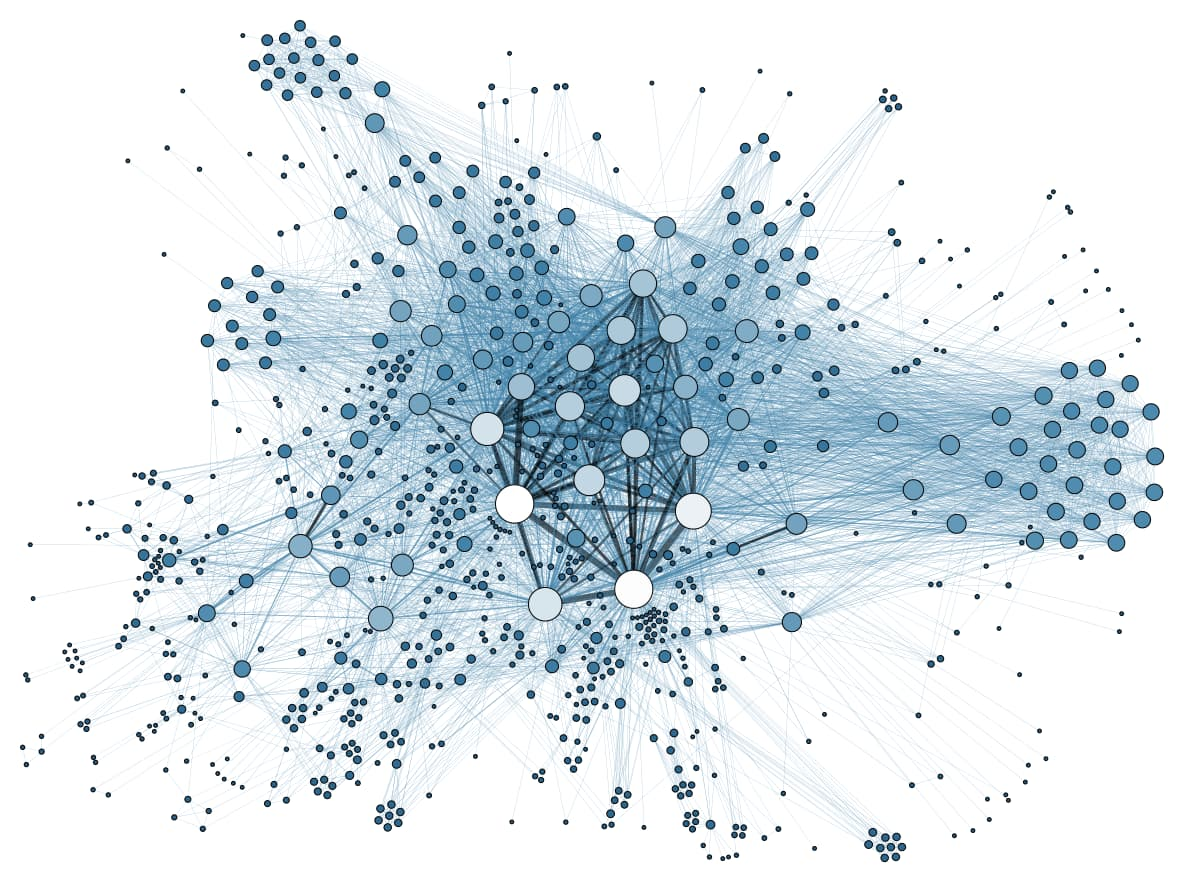
\includegraphics[width=0.95\textwidth]{src/images/chapter2/graph-social-network.jpg}
    \caption{Một ví dụ về đồ thị}
    \label{fig:graph}
\end{figure}

\bigbreak\noindent
Đồ thị có thể được phân loại theo những hướng sau:

\begin{itemize}
    \item \textit{Đồ thị đồng nhất và không đồng nhất}: Trong đồ thị đồng nhất, các nút và cạnh có cùng một loại, có chung các loại thuộc tính. Ngược lại, đồ thị không đồng nhất bao gồm nhiều loại nút khác nhau với thuộc tính riêng biệt của mỗi loại, tương tự như vậy với cạnh.
    \item \textit{Đồ thị vô hướng và có hướng}: Đồ thị vô hướng có các cạnh không hướng, chỉ biểu thị sự kết nối giữa hai nút. Trái lại, đồ thị có hướng có các cạnh đều có hướng từ một cạnh này sang cạnh khác, điều này cung cấp thông tin chi tiết hơn so với đồ thị không hướng. Mỗi cạnh trong đồ thị không hướng cũng có thể được xem như hai cạnh có hướng.
    \item \textit{Đồ thị tĩnh và động}: Một đồ thị được xem là đồ thị tĩnh nếu các thuộc tính hay cấu trúc đồ thị không đổi theo thời gian, và nếu ngược lại sẽ được xem là đồ thị động.
\end{itemize}

\bigbreak\noindent
Đồ thị là một dạng cấu trúc dữ liệu khó phân tích với độ phức tạp cao, không có hình dạng cố định, có kích thước biến đổi với các nút không được sắp xếp, trong đó các nút có thể có số lượng hàng xóm khác nhau, cùng với nhiều loại thuộc tính riêng biệt. Các thuật toán học sâu truyền thống chỉ chuyên dụng cho các loại dữ liệu đơn giản, ví dụ như hình ảnh, văn bản và âm thanh, ...

\bigbreak\noindent
\textbf{Mạng GNN}
\bigbreak\noindent
Mạng GNN là một loại mạng nơ-ron nhân tạo được thiết kế để làm việc với dữ liệu có cấu trúc đồ thị. Mạng GNN có khả năng xử lý và khám phá thông tin trên đồ thị một cách hiệu quả, đồng thời giữ nguyên sự tổ chức và mối quan hệ giữa các yếu tố trong đồ thị (các đỉnh, cạnh và ngữ cảnh toàn cục). Mạng GNN cung cấp khả năng thực hiện các công việc ở mức độ nút, mức độ cạnh và mức độ toàn đồ thị một cách dễ dàng. Mạng GNN có khả năng thực hiện các công việc như sau: biểu diễn/phân loại đồ thị/nút/cạnh, phân cụm, sinh đồ thị, ... 

\bigbreak\noindent
Ý tưởng chính của GNN là việc sử dụng truyền thông điệp theo cặp, trong đó các nút và các cạnh trong đồ thị cập nhật biểu diễn của chúng bằng cách trao đổi thông tin với các hàng xóm của mình, từ đó đưa ra dự đoán và phân loại trên dữ liệu đồ thị. Mô hình chung nhất của quá trình truyền thông điệp có trình tự như sau:

\begin{itemize}
    \item Các nút hoặc cạnh sẽ nhận được các thông điệp (hay còn được gọi là vectơ biểu diễn) từ các nút hoặc cạnh hàng xóm (tuỳ thuộc vào thuật toán truyền thông tin được sử dụng).
    \item Tổng hợp tất cả các thông điệp sử dụng thông qua một hàm tổng hợp (như tổng, trung bình cộng, ...)
    \item  Sau khi kết hợp thông điệp, quá trình này có thể bao gồm việc sử dụng các hàm kích hoạt phi tuyến để tạo ra biểu diễn cập nhật cho nút hay cạnh dựa trên thông điệp được tổng hợp.
\end{itemize}

\bigbreak\noindent
Có nhiều loại mạng GNN khác nhau dựa trên cách chúng truyền thông điệp, một số có thể kể đến như là:

\begin{itemize}
    \item \textit{GCN (Graph Convolution Network)} \cite{kipf2016semi}: Đây là một dạng mạng GNN cơ bản, được sử dụng rộng rãi trong xử lý đồ thị. GCN kết hợp thông tin từ các nút láng giềng để cập nhật đại diện cho mỗi nút.

    \item \textit{GAT (Graph Attention Network)} \cite{velivckovic2017graph}: Mạng GAT sử dụng cơ chế chú ý (attention) để xác định tầm quan trọng của các nút láng giềng trong quá trình cập nhật đại diện của mỗi nút. Điều này giúp mạng tập trung vào thông tin quan trọng nhất trong đồ thị.

    \item \textit{GraphSAGE (SAmple and aggreGatE)} \cite{hamilton2017inductive}: Mạng GraphSAGE sử dụng một quá trình lấy mẫu ngẫu nhiên các nút láng giềng và tổng hợp thông tin từ chúng để cập nhật đại diện cho mỗi nút. Điều này giúp mạng học được thông tin từ toàn bộ đồ thị.

    \item \textit{GAE (Graph Auto Encoder)} \cite{kipf2016variational}: Mạng GAE kết hợp cả thông tin từ nút láng giềng và thông tin về cạnh trong quá trình cập nhật đại diện cho mỗi nút. Điều này cho phép mạng học được sự tương tác giữa các nút và cạnh trong đồ thị.
\end{itemize}

\section{Học liên kết}

\subsection{Tổng quan về học liên kết}

AI ngày càng được ứng dụng rộng rãi vào trong mọi mặt của đời sống, góp phần không nhỏ trong sự thúc đẩy sự phát triển của xã hội, đồng nghĩa với đó là việc huấn luyện các mô hình AI đang được tiến hành ngày một nhiều. Việc huấn luyện đòi hỏi một lượng dữ liệu rất là lớn, đòi hỏi việc duy trì và làm mới dữ liệu huấn luyện. Tuy nhiên từ đây lại nảy sinh ra hai vấn đề: thứ nhất, việc dựa vào các nguồn dữ liệu nội tại của một cá nhân hoặc tổ chức thường không thể đầy đủ vì thiếu về cả số lượng lẫn sự đa dạng; thứ hai, các dữ liệu được chia sẻ thường không đảm bảo về chất lượng do những quan ngại về tính riêng tư cùng với đó là các chính sách chia sẻ dữ liệu của các tổ chức.

\bigbreak\noindent
Học liên kết nổi lên như là một giải pháp cho các vấn đề liên quan tới dữ liệu huấn luyện nói trên nhờ vào khả năng huấn luyện phi tập trung mà không cần phải chia sẽ dữ liệu nội bộ. Các bên đồng ý tham qua quá trình học liên kết sẽ huấn luyện mô hình sử dụng chính dữ liệu của mình, sau khi hoàn tất, các mô hình của các bên tham gia được tổng hợp thành mô hình chung. Các bên đều có thể sử dụng mô hình chung và hưởng lợi từ nó. 

\subsection{Quá trình huấn luyện}

\begin{figure}[h]
    \centering
    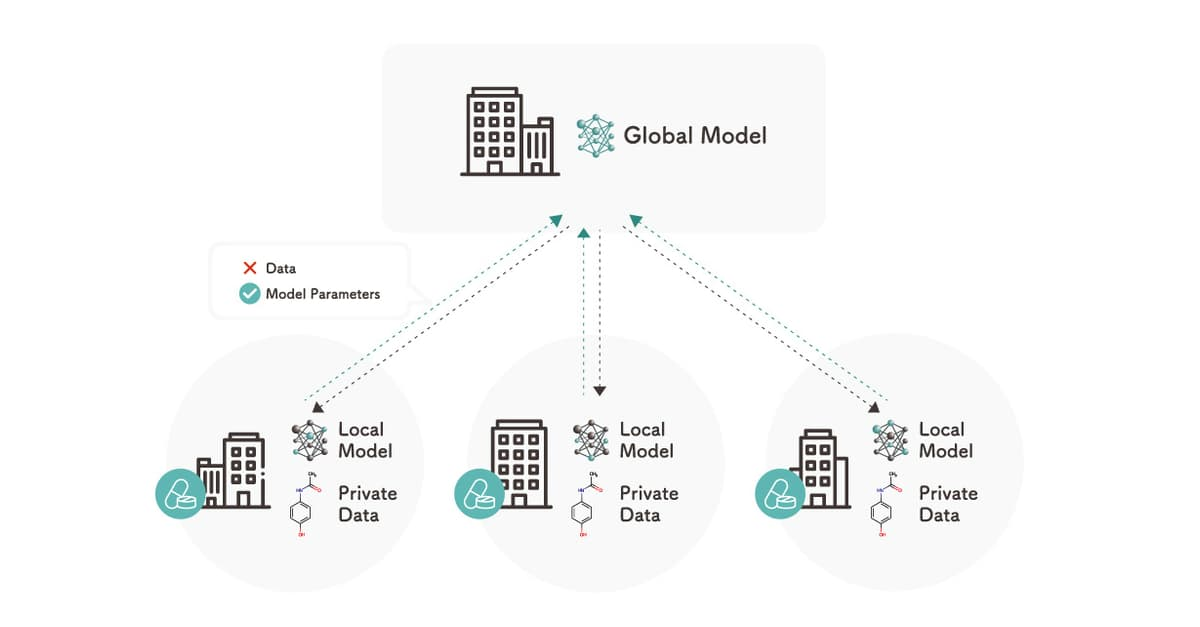
\includegraphics[width=\textwidth]{src/images/chapter2/federated-learning.jpg}
    \caption{Mô hình học liên kết tổng quát}
    \label{fig:federated-learning}
\end{figure}

\bigbreak\noindent
Như được mô tả trong \textbf{Hình \ref{fig:federated-learning}}, quá trình huấn luyện bao gồm các bên tham gia cùng với một trung tâm huấn luyện, đây là nơi tổng hợp các mô hình cục bộ thành mô hình chung. Việc huấn luyện bao gồm một hoặc nhiều vòng, với chi tiết mỗi vòng như sau:

\begin{itemize}
    \item \textit{(1) Khởi tạo}: Một mô hình học máy được chọn và khởi tạo các tham số để thực hiện huấn luyện. Sau đó, các thành viên tham gia sẽ sẵn sàng thực hiện huấn luyện. Đây là việc chỉ xảy ra ở vòng đầu tiên của quá trình huấn luyện, và các vòng sau sẽ bắt đầu từ \textit{(2) Chọn thành viên tham gia}.
    
    \item  \textit{(2) Chọn thành viên tham gia}: Một phần các thành viên sẽ được chọn và tham gia thực hiện huấn luyện còn các thành viên còn lại sẽ đợi vòng tiếp theo.
    
    \item \textit{(3) Huấn luyện}: Các thành viên được chọn sẽ nhận được tham số ban đầu của mô hình được gửi từ trung tâm huấn luyện, sau đó huấn luyện dựa trên dữ liệu nội tại của mỗi thành viên.
    
    \item \textit{(4) Cập nhật mô hình}: Các thành viên sau khi hoàn thành huấn luyện thì sẽ gửi mô hình của mình lên trung tâm huấn luyện. Trung tâm huấn luyện sẽ tổng hợp các mô hình và cập nhập mô hình chung. Sau đó các tham số của mô hình chung mới sẽ được gửi về lại cho các thành viên. Từ đây, có thể bắt đầu vòng tiếp theo của việc huấn luyện.
    
    \item \textit{(5) Hoàn tất}: Khi mà điều kiện dừng được đáp ứng (hoàn thành số vòng huấn luyện, mô hình đã hội tụ, ...) thì trung tâm huấn luyện sẽ tổng hợp tất cả các cập nhật và hoàn tất việc huấn luyện.
\end{itemize}

\bigbreak\noindent
Hiện nay có nhiều thuật toán tổng hợp đã được nghiên cứu và sử dụng cho học liên kết như FedAvg \cite{mcmahan2017communication}, FedSGD, Fed+ \cite{yu2020fed+}, ... Trong đề tài này, chúng tôi sử dụng FedAvg cho học liên kết. Chi tiết sẽ được chúng tôi trình bày tại \textbf{Mục \ref{sec:FL-model}}.

%----------------------------------------------------------------------------------------
%	SECTION 4
%----------------------------------------------------------------------------------------

\section{Học máy khả giải}

\subsection{Tổng quan}

Các mô hình AI đang được áp dụng rộng rãi trong nhiều lĩnh vực đời sống như y tế, tài chính, giáo dục, và cả an ninh thông tin. Tuy nhiên, các mô hình AI ngày càng trở nên phức tạp để có thể đáp các nhu cầu phân tích các loại dữ liệu khác nhau nhưng kéo theo đó là sự giảm mạnh ở khả năng diễn giải của mô hình. Đặc biệt là khi các mô hình AI ngày nay chủ yếu sử dụng các mạng nơ-ron nhân tạo nhằm làm tăng hiệu suất của mô hình. Tuy nhiên, các mạng nơ-ron này thường rất phức tạp và khó giải thích khi so sánh với các thuật toán truyền thống như cây quyết định, hồi quy tuyến tính,... như được mô tả trong \textbf{Hình \ref{fig:xai-complexity}}. Điều này khiến cho người dùng cuối và các nhà phát triển gặp khó khăn trong việc hiểu và xác minh các quyết định được đưa ra bởi các mô hình. Hệ quả là làm giảm khả năng phát triển, gỡ lỗi các mô hình cũng như khả năng áp dụng các mô hình học máy trong các lĩnh vực yêu cầu sự minh bạch và giải thích như sức khỏe, pháp luật hay an toàn thông tin. 

\begin{figure}[h]
    \centering
    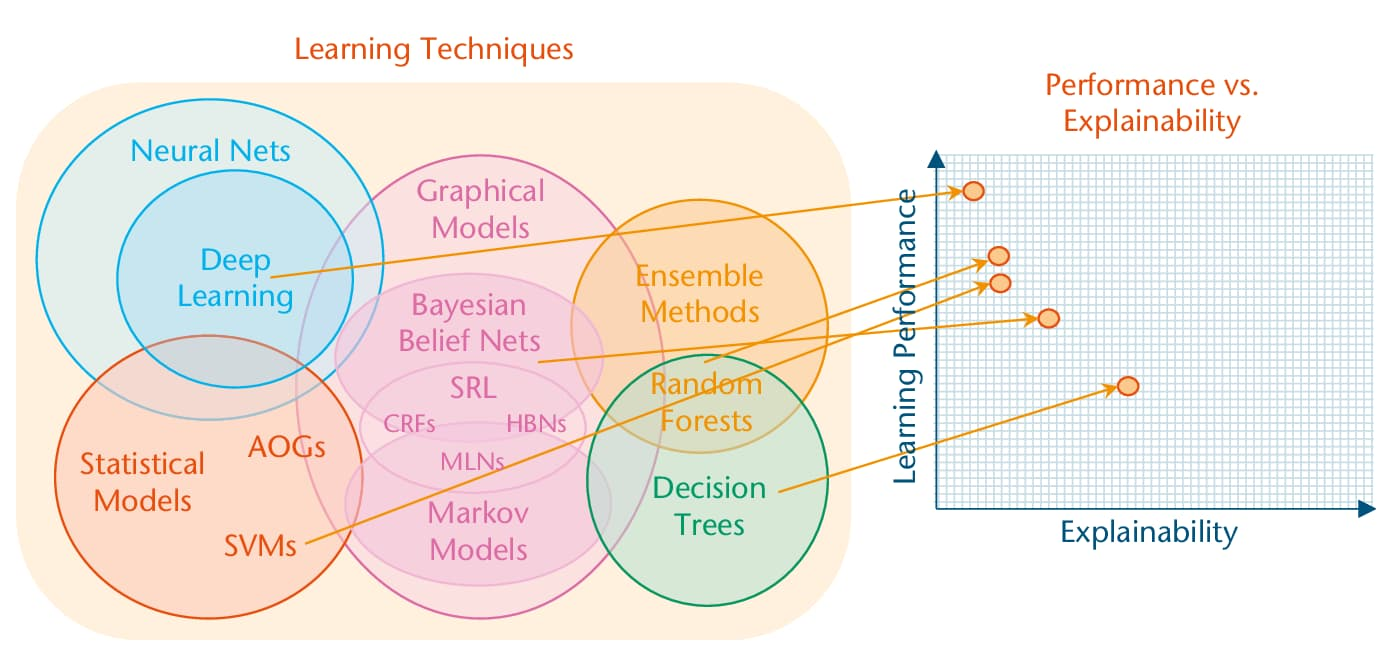
\includegraphics[width=\textwidth]{src/images/chapter2/xai-complexity.jpg}
    \caption[Tương quan giữa hiệu suất và khả năng diễn giải của các mô hình máy học]{Tương quan giữa hiệu suất và khả năng diễn giải của các mô hình máy học \cite{gunning2019darpa}}
    \label{fig:xai-complexity}
\end{figure}

\bigbreak\noindent
Các phương pháp học máy khả giải ra đời với sứ mệnh giải thích tại sao các thuật toán máy học lại đưa ra các quyết định như thế theo cách mà con người có thể hiểu được. Thông qua học máy khả giải, chúng ta có thể đánh giá các tiêu chí quan trọng khác của một mô hình học máy như: sự công bằng, sự tin cậy và khả năng chống nhiễu, sự riêng tư, sự khả dụng và sự tin cậy \cite{doshi2017towards}.
\bigbreak\noindent
%Từ việc có thể kiểm tra được các tiêu chí trên chúng ta có thể gỡ lỗi mô hình, phát triển mô hình với hiệu suất cao hơn và nâng cao lòng tính của người dùng đối với các mô hình AI. Chính những khía cạnh trên đã thúc đẩy sự phát triển của lĩnh vực học máy khả giải với mục tiêu lý giải được cách các mô hình AI hiện hành hoạt động và đưa ra dự đoán.


%Học máy khả giải là một lĩnh vực trong đó các mô hình máy học được thiết kế để có khả năng giải thích rõ ràng và minh bạch về quá trình ra quyết định hoặc sử dụng các thuật toán. Mục tiêu của học máy khả giải là giúp con người hiểu được lý do mô hình học máy đưa ra các quyết định và dự đoán cụ thể.

%Trong học máy thông thường, các mô hình như mạng nơ-ron sâu (deep neural networks) thường có khả năng dự đoán mạnh mẽ, nhưng việc giải thích cách mô hình đưa ra quyết định trở nên khó khăn. Học máy khả giải tập trung vào việc xây dựng các mô hình dễ hiểu, như cây quyết định hoặc hồi quy tuyến giúp con người có thể theo dõi và hiểu được quá trình ra quyết định của mô hình.

%\begin{figure}[h]
%    \centering
%    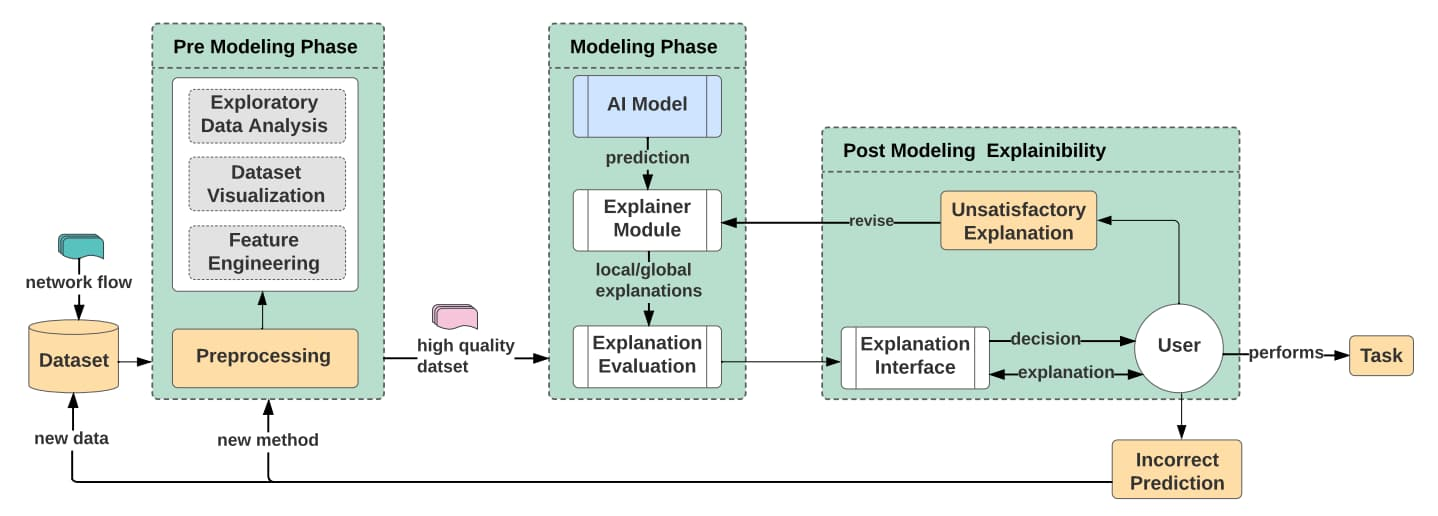
\includegraphics[width=\textwidth]{src/images/chapter2/xai-achitecture.jpg}
%    \caption{Kiến trúc cơ bản của mô hình sử dụng học máy khả giải}
%    \label{fig:xai-achitecture}
%\end{figure}

\subsection{Phân loại}
Chúng ta có thể chia các phương pháp được sử dụng trong học máy khả giải theo nhiều tiêu chí khác nhau tùy thuộc vào độ phức tạp của mô hình, phạm vi giải thích và loại mô hình cần được giải thích. Cụ thể, chúng ta có thể chia các phương pháp sử dụng trong học máy khả giải theo các tiêu chí sau:
\bigbreak\noindent
\textbf{Nội tại (intrinsic) và sau huấn luyện (post-hoc)}
\begin{itemize}
    \item \textit{Nội tại}: Thiết kế các mô học có khả năng giải thích rõ ràng và minh bạch về quá trình ra quyết định của chúng. Các mô hình này thường được thiết kế dựa trên thuật toán đơn giản và có khả năng tự diễn giải cao như cây quyết định hoặc hồi quy tuyến tính. Tuy nhiên, do chỉ dựa trên các thuật toán đơn giản nên các mô hình này thường gặp khó khăn với các dữ có nhiều thuộc tính với các mối quan hệ phức tạp.
    \item \textit{Sau huấn luyện}: Tập trung vào việc sử dụng các thuật toán, các phương pháp diễn giải nhằm tạo ra giải thích cho mô hình sau khi huấn luyện, thường là các mạng nơ-ron phức tạp. Các kỹ thuật như SHAP, LIME, Grad-CAM, ... đều thuộc loại này. Tuy nhiên, các phương pháp loại này thường có độ phức tạp tương đối cao, chịu ảnh hưởng của nhiều yếu tố và mất thêm thời gian để tính toán.
\end{itemize}

\bigbreak\noindent
\textbf{Cục bộ (local) và toàn cục (global)}
\begin{itemize}
    \item \textit{Cục bộ}: Tập trung vào việc hiểu và giải thích dự đoán của mô hình cho một trường hợp dữ liệu cụ thể. ác phương pháp thuộc loại này thường tìm hiểu các yếu tố quan trọng và đặc trưng được mô hình coi trọng nhất để đưa ra quyết định phân loại cho trường hợp dữ liệu đó. Các phương pháp giải thích tiêu biểu thuộc này là: LIME, SHAP, GNNExplainer, Grad-CAM,... Tuy nhiên, vì chỉ tập trung vào một dự đoán đơn lẻ, giải thích cụ bộ thường thiếu đi khả năng tổng quát hóa, khả năng hiểu về mối quan hệ giữa các dự đoán của mô hình.
    \item \textit{Toàn cục}: Giải thích toàn cục tập trung vào việc hiểu và giải thích cách hoạt động của mô hình học máy trên toàn bộ tập dữ liệu. Nó tìm hiểu các mô hình, thuật toán và đặc trưng tổng quát mà mô hình sử dụng để đưa ra quyết định phân loại. Giải thích toàn cục giúp chúng ta có cái nhìn tổng quan về cách mô hình hoạt động và tại sao nó đưa ra các quyết định phân loại như vậy trên toàn bộ dữ liệu. Các phương pháp giải thích tiêu biểu thuộc này là: PDP \cite{greenwell2017pdp} (Partial Dependence Plot), GAM \cite{ibrahim2019global} (Global Attribution Mapping),... Tuy nhiên, giải thích toàn cục cũng có những hạn chế như sự trừu tượng, mất mát thông tin chi tiết, ...
\end{itemize}

\bigbreak\noindent
\textbf{Mô hình cụ thể (specific-model) và không phụ thuộc vào mô hình (agnostic-model)}
\begin{itemize}
    \item \textit{Mô hình cụ thể}: Phương pháp giải thích được thiết kế dựa trên cấu trúc và thông tin của một loại mô hình học hoặc một tập các mô hình nhất định, thông qua việc sử dụng kiến thức về mô hình, thuật toán và quy trình học để giải thích cách mô hình đưa ra quyết định. Grad-CAM là các ví dụ tiêu cho loại này. Tuy nhiên, do chỉ phù hợp với một số dạng mô hình nhất định nên các phương pháp loại này thường hạn chế về phạm vi diễn giải.
    \item \textit{Không phụ thuộc vào mô hình}: Phương pháp được thiết kế có giải thích cho bất cứ mô hình nào và thường được áp dụng đối với mô hình sau huấn luyện. Tiêu biểu là các phương pháp như: PDP, GAM, SHAP, LIME, ...
\end{itemize}

\subsection{Đánh giá khả năng diễn giải} \label{sec:interpretability-metric}

Hiện vẫn chưa có sự đồng nhất rõ ràng về ý nghĩa của thuật ngữ ``interpretability" trong lĩnh vực học máy. Đồng thời, việc đo lường khả năng diễn giải cũng chưa có phương pháp đo rõ ràng. Tuy nhiên, đã có một số nghiên cứu ban đầu về vấn đề này và đã đề xuất một số phương pháp để đánh giá. Như trong nghiên cứu của Doshi-Velez và các cộng sự \cite{doshi2017towards}, các tác giả đã chia các phương pháp đánh giá khả năng diễn giải của một giải thích thành ba loại như trong \textbf{Hình \ref{fig:explanation-metric}}.

\begin{figure}[h]
    \centering
    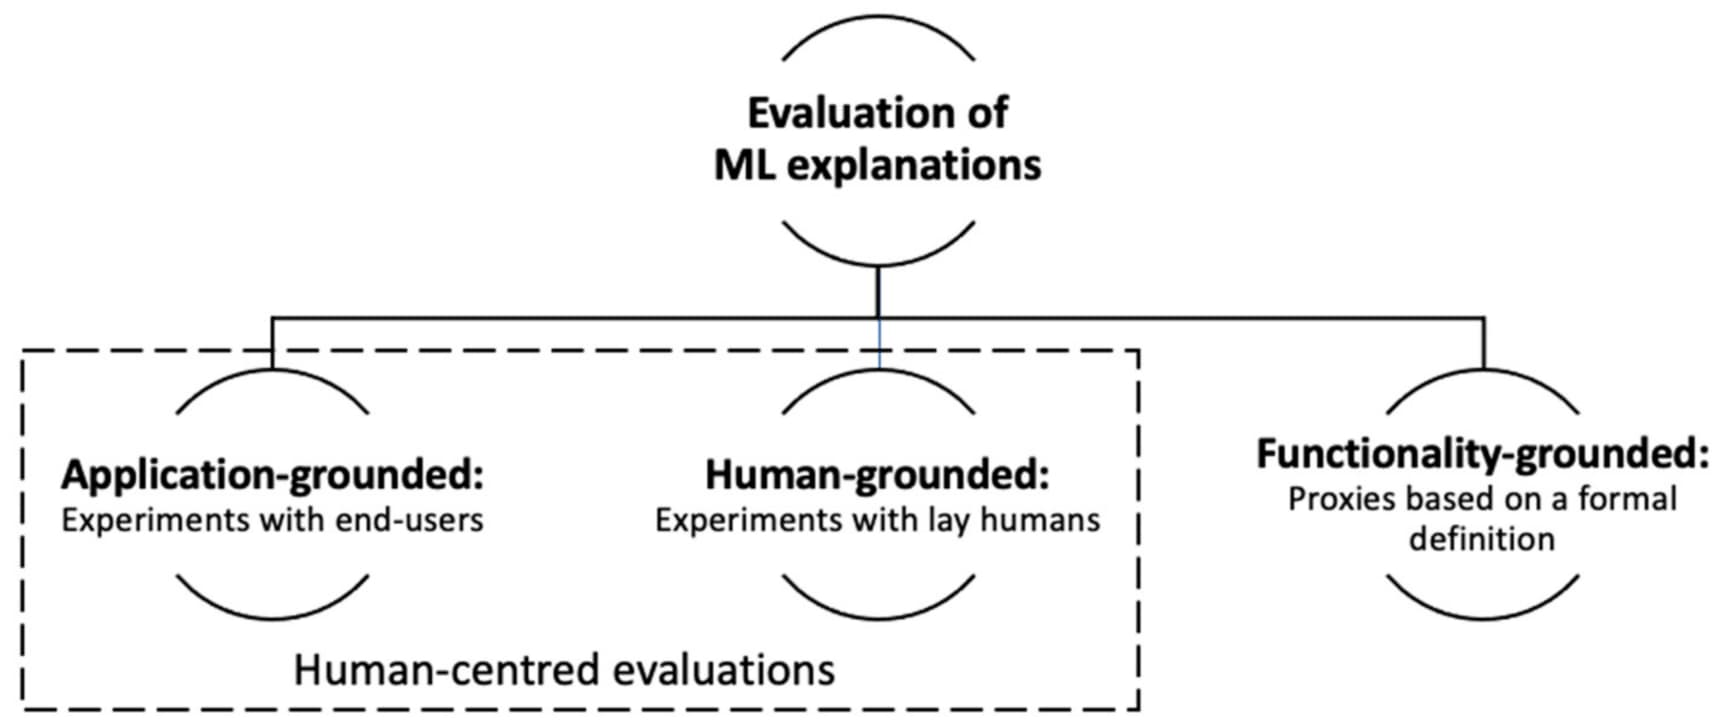
\includegraphics[width=0.8\textwidth]{src/images/chapter2/explanation-metric.jpg}
    \caption{Các phương pháp đánh giá khả năng diễn giải của giải thích}
    \label{fig:explanation-metric}
\end{figure}

\begin{itemize}
    \item \textit{Đánh giá ở mức độ ứng dụng (application-grounded evaluation)}: Đánh giá dựa trên sự tác động của quá trình giải thích đối với chuyên gia hoặc người dùng cuối có kiến thức chuyên với một công việc đã được xác định trước. Giả sử chúng ta sử dụng một phương pháp học máy khả giải để tìm ra các nhân tố quan trọng ảnh hưởng đến quyết định của một hệ thống IDS sử dụng một mô hình học sâu để dự đoán tấn công mạng. Ở mức độ ứng dụng, chúng ta sẽ đưa các giải thích được tạo cho các chuyên gia để đánh giá chất lượng của giải thích. Đây là phương pháp có hiệu suất cao cũng như ít sai số nhất. Tuy nhiên, phương pháp đánh giá này đòi hỏi phương pháp phải hoạt động được với mô hình dự đoán toán công mạng và người đánh giá phải có kiến thức chuyên môn về tấn công mạng.
    \item \textit{Đánh giá ở mức độ con người (human-grounded evaluation)}: Tương tự với \textit{đánh giá căn cứ vào ứng dụng} nhưng những người kiểm tra trong trường hợp này không cần phải là một chuyên gia trong lĩnh vực. Điều này cho phép chúng ta có thể chọn người đánh giá từ một tập rộng hơn, từ đó giảm chi phí đánh giá. Thêm vào đó, vì được thí nghiệm trên tạp người dùng cuối rộng hơn này kết quả đánh giá giải thích cũng sẽ tổng quát hơn. Tuy nhiên, phương pháp đánh giá này sẽ kém chính xác trong một số thí nghiệm đòi hỏi tính chuyên môn cao. 
    \item \textit{Đánh giá ở mức độ chức năng (functionality-grounded evaluation)}: không yêu cầu bất kỳ thí nghiệm nào liên quan đến con người, mà thay vào đó sử dụng các định nghĩa toán học cụ thể, rõ ràng đã được kiểm chứng và chấp thuận để đánh giá chất lượng của một phương pháp giải thích. Ví dụ với cây quyết định, cây có độ sâu thấp hơn có khả năng diễn giải tốt hơn. Ngoài ra, phương pháp này cũng được sử dụng trong các thí nghiệm mà các phương pháp đánh giá dựa trên con người không thể được áp dụng vì một số lý do (ví dụ như các yếu tố đạo đức) hoặc khi phương pháp đề xuất chưa đủ tường minh để có thể đánh giá bởi con người.
\end{itemize}

\subsection{Giá trị Shapley}
Giá trị Shapley \cite{winter2002shapley} là một phương pháp tính toán giá trị đóng góp của mỗi người chơi trong một trò chơi hợp tác. Trong đó, một trò chơi hợp tác là một trò chơi được hiểu là có sự tham gia của hai hay nhiều người trở lên nhằm đạt được một giải thưởng nào đó. Giá trị Shapley được tính toán bằng cách xem xét tất cả các tổ hợp có thể có của các người chơi và tính toán trung bình tất cả sự tăng giá trị phần thưởng trên tất cả mọi tổ hợp người chơi mỗi khi có người chơi mới tham gia vào. Kết quả là một phân phối công bằng của giá trị tạo ra, trong đó mỗi người chơi nhận được một phần trăm công bằng dựa trên đóng góp của họ.
\bigbreak\noindent
Giả sử một nhóm học sinh (được ký hiệu là $N$) gồm $M$ thành viên cần phối hợp để hoàn thành một dự án. Bởi vì đóng góp của mỗi thành viên trong nhóm là không đồng đều nên chúng ta cần phải làm sao đó để phân phối công bằng điểm của tổng dự án $v=v(T)$ cho từng thành viên trong nhóm. Để giải quyết vấn đề này, chúng ta sẽ sử dụng giá trị Shapley $\varphi_i(v)$ để đại diện cho cống hiến của thành viên thứ $i$ trong nhóm và $\varphi_i(v)$ có thể được xác định theo công thức sau:

%\begin{enumerate}
%    \item Cho một người chơi $i$ cần được tính toán Xác định tất cả các tổ hợp chứa người chơi cần tính toán đóng góp của người đó có thể có của tất cả các người chơi, từ tập rỗng cho đến tập hợp chứa tất cả các người chơi.

%    \item Đối với mỗi tập hợp con, tính toán giá trị kỳ vọng của trò chơi khi có sự tham gia của tập hợp con đó. Đây là giá trị kỳ vọng của trò chơi khi tất cả các người chơi trong tập hợp con đó tham gia cùng với các người chơi không nằm trong tập hợp con đó.

%    \item Đối với mỗi người chơi, tính toán giá trị đóng góp của người chơi đó trong từng tập hợp con. Giá trị đóng góp của một người chơi là sự khác biệt giữa giá trị kỳ vọng của trò chơi khi có sự tham gia của người chơi đó và giá trị kỳ vọng của trò chơi khi không có sự tham gia của người chơi đó.

%    \item Tổng hợp các giá trị đóng góp của tất cả các tập hợp con để tính toán giá trị Shapley của từng người chơi. Giá trị Shapley của một người chơi là trung bình của tất cả các giá trị đóng góp của người chơi đó.
%\end{enumerate}

%\bigbreak\noindent
%Về mặt công thức toán học, ta xét một trò chơi hợp tác gồm tập $N$ gồm $n$ người chơi. $S$ là tập hợp người chơi con của $N$. $v$ đại diện cho một hàm giá trị, thường được gọi là hàm giá trị của trò chơi. Hàm giá trị này đo lường giá trị kỳ vọng của trò chơi khi có sự tham gia của các người chơi. Ta có công thức tính giá trị Shapley của người chơi $i$ như sau:

\begin{equation} \label{eq:shapley-value-raw}
\varphi_i(v) = \frac{1}{M}\sum_{S \subseteq N \setminus \{i\}} \frac{1}{\binom{M - 1}{|S|}}\left[ v(S \cup \{i\}) - v(S) \right]
\end{equation}
Trong đó, $S$ là nhóm con thuộc $N$ không chứa thành viên thứ $i$, $|S|$ là số lượng thành viên trong tập $S$, $\left[ v(S \cup \{i\}) - v(S) \right]$ là lượng điểm thay đổi khi thành viên thứ $i$ tham gia vào nhóm $S$ (đóng góp của thành viên thứ $i$ trong nhóm $v(S \cup \{i\})$) và $\binom{M - 1}{|S|}$ là tổ hợp chập $|S|$ của $M-1$ phần tử (được dùng để tính trọng số cho đóng góp của thành viên $i$ trong nhóm $S$).

\bigbreak\noindent
\textbf{Công thức \ref{eq:shapley-value-raw}} có thể được viết lại, sau khi khai triển $\binom{n - 1}{|S|}$, như sau:

\begin{equation} \label{eq:shapley-value}
\varphi_i(v) = \sum_{S \subseteq N \setminus \{i\}} \frac{|S|!(n-|S|-1)!}{n!} \left[ v(S \cup \{i\}) - v(S) \right]
\end{equation}
\bigbreak\noindent

%\textbf{Giá trị Shapley đối với học máy khả giải}
\bigbreak\noindent
Với khả năng tính toán đóng góp của các phần tử trong một tập hợp, giá trị Shapley có thể được áp dụng trong nhiều lĩnh vực, trong đó có học máy khả giải. Giá trị Shapley được áp dụng vào học máy khả giải nhằm đo lường đóng góp của từng thuộc tính vào dự đoán của mô hình. Ý tưởng cơ bản là ta có thể giải thích một dự đoán bằng cách xem mỗi giá trị thuộc tính là một ``người chơi" trong một trò chơi hợp tác, trong đó dự đoán là phần thưởng, từ đó đưa ra được sự đóng góp của mỗi thuộc tính. Giá trị Shapley không chỉ đánh giá giá trị đóng góp của mỗi thuộc tính độc lập mà còn xem xét cách chúng tương tác với nhau để đưa ra một giải thích toàn diện hơn về quyết định của mô hình. Ngoài ra, giá trị Shapley cũng cho phép so sánh và giải thích theo hướng tương phản. Bên cạnh đó, Ta cũng có thể so sánh giải thích được giải thích của một dự đoán với trung bình của toàn bộ tập dữ liệu, hoặc so sánh với một tập con hoặc một điểm dữ liệu cụ thể. Điều này tạo ra sự linh hoạt trong việc giải thích và giúp phát hiện sự khác biệt quan trọng giữa các trường hợp. Nhờ vào tính ứng dụng trên, giá trị Shapley được sử dụng bởi nhiều phương pháp học máy khả giải, tiêu biểu trong đó là bộ khung SHAP \cite{lundberg2017unified}.

\bigbreak\noindent
Tuy nhiên, khi ứng dụng giá trị Shapley trong học máy khả giải cũng có những hạn chế nhất định. Đầu tiên là về thời gian tính toán, với mỗi thuộc tính, ta phải tính toán sự đóng góp với tất cả các tập con không có thuộc tính hiện tại. Với các ngữ cảnh thực tế, các mô hình có thể có đến vài ngàn hoặc vài triệu thuộc tính. Điều này khiến cho việc tính toán là cực kỳ tốn kém và buộc phải sử dụng các phương pháp xấp xỉ giá trị Shapley như KernelSHAP hoặc GradientSHAP thuộc bộ khung SHAP.% Ngoài ra, giá trị Shapley đơn giản chỉ là một con số thể hiện sự đóng góp. Nó không cung cấp khả năng đưa ra những phát biểu về sự thay đổi trong dự đoán khi thay đổi giá trị thuộc tính đầu vào, ví dụ như ``Nếu giá trị của thuộc tính là 5 thì dự đoán sẽ là 10".

\subsection{LIME} \label{sec:lime}
LIME \cite{9825734} là một phương pháp giải thích mô hình không phụ thuộc vào mô hình dự đoán. Nó được sử dụng để giải thích dự đoán của các mô hình học máy đen hộp, bao gồm cả mô hình học sâu thông qua việc sử dụng một mô hình thay thế cục bộ. LIME tập trung vào việc huấn luyện các mô hình thay thế cục bộ sao cho chúng có thể tính toán xấp xỉ các dự đoán của mô hình gốc đối với một mẫu dữ liệu nhất định, từ đó, giải thích dự đoán của mô hình thay thế cục bộ đơn giản thay vì cố gắng hiểu dự đoán thông qua mô hình gốc phức tạp.

\bigbreak\noindent
Về mặt ý tưởng, hãy tưởng tượng rằng chúng ta chỉ có một mô hình hộp đen và chúng ta chỉ có thể đưa dữ liệu vào và nhận được dự đoán từ mô hình đó. Mục tiêu của chúng ta là xác định các thuộc tính có ảnh hưởng lớn đến mộ dư đoán cụ thể của mô hình hộp đen. Để làm được điều đó, LIME sẽ thực hiện kiểm tra sự biến đổi trong dự đoán từ mô hình hộp đên khi chúng ta đưa các biến thể của dữ liệu vào. Đầu tiên, LIME tạo ra một tập dữ liệu mới bao gồm các mẫu bị nhiễu và các dự đoán từ mô hình hộp đen tương ứng với từng mẫu. Trên tập dữ liệu mới này, LIME huấn luyện một mô hình có khả năng diễn giải cao (thường là các mô hình đơn giản như mô hình hồi quy tuyến tính như mô tả trong \textbf{Hình \ref{fig:lime}} hoặc cây quyết định). Ngoài ra, mô hình giải thích cần đảm bảo dự đoán xấp xỉ giống với mô hình toàn cục ở mức cục bộ nhưng có thể không xấp xỉ tốt ở mức toàn cục (loại chính xác này còn được gọi là tính chính xác cục bộ). Nhằm đảm bảo độ chính xác cục bộ trên, các mẫu dữ liệu sẽ được đánh trọng số dựa trên sự gần gũi của các mẫu được lấy mẫu đến điểm dữ liệu quan tâm trong quá trình huấn luyện. Cuối cùng, chúng ta có thể thực hiện giải thích một dự đoán cụ thể của mô hình hộp đen thông qua mô hình cục bộ có khả năng diễn giải cao.

%\bigbreak\noindent
%Ý tưởng cơ bản của LIME là tạo ra bộ dữ liệu huấn luyến mới bao gồm các mẫu dữ liệu nhiễu hoặc các mẫu xung quanh  sẽ huấn luyện một mô hình thay thế cục bộ bằng cách huấn luyện  xác định độ quan trọng của các thuộc tính đầu vào đối với dự đoán của một mô hình học máy cụ thể trong một vùng xung quanh dữ liệu đầu vào cụ thể. Nó hoạt động bằng cách xây dựng một mô hình giải thích cục bộ đơn giản (thường là mô hình hồi quy tuyến tính hoặc cây quyết định) cho một mẫu dữ liệu cụ thể xung quanh điểm đó, như trong \textbf{Hình \ref{fig:lime}}. Mô hình giải thích cục bộ này có thể dễ dàng được giải thích và hiểu được.

\begin{figure}[h]
    \centering
    \includegraphics[width=\textwidth]{src/images/chapter2/lime.jpg}
    \caption[Ví dụ về hướng tiếp cận của LIME]{Ví dụ về hướng tiếp cận của LIME sử dụng một mô hình quy tuyến tính đơn giản để giải thích cho một dự đoán được tạo bởi một mô hình toàn cục phức tạp}
    \label{fig:lime}
\end{figure}

\bigbreak\noindent
Một giải thích cho một dự đoán cụ thể từ mô hình toàn cục $f$ cho một điểm dữ liệu $x$ sẽ được biểu diễn theo phương pháp của LIME như sau:

\begin{equation}\label{eq:lime-explanation}
explanation(x) = argmin_{g \in G} \mathcal{L}(f, g, \Pi_x) + \Omega(g)
\end{equation}
\bigbreak\noindent
Trong đó, $g$ là mô hình thay thế cục bộ (ví dụ như có thể là mô hình hồi quy tuyến tính), $L$ là hàm mất mát mà ta phải tối ưu để tìm ra $g$ (ví dụ như hàm sai số bình phương trung bình), trong khi, giữ độ phức tạp của mô hình $\Omega(g)$ ở mức thấp (ví dụ như ưu tiên ít thuộc tính hơn). $G$ là tập hợp các giải thích có thể (ví dụ như tất cả các mô hình hồi quy tuyến tính có thể có) và hàm $\Pi_x$ dùng để xác định trọng số của các điểm dữ liệu xung quanh $x$ mà chúng ta xem xét cho giải thích. Trong thực tế, LIME chỉ tối ưu phần mất mát và người dùng phải tự xác định độ phức tạp, ví dụ như bằng cách chọn số lượng đặc trưng tối đa mà mô hình hồi quy tuyến tính có thể sử dụng.

\subsection{GNNExplainer} \label{sec:gnnexplainer}

GNNExplainer là một phương pháp học máy khả giải được phát triển bởi Ying và các cộng sự. Ý tưởng chính ban đầu của GNNExplainer là việc xác định đóng góp của các nút của đồ thị và các con đường truyền thông điệp quan trọng trong việc đưa ra quyết định như mô tả trong \textbf{Hình \ref{fig:gnn_explainer}}.

\begin{figure}[ht]
    \centering
    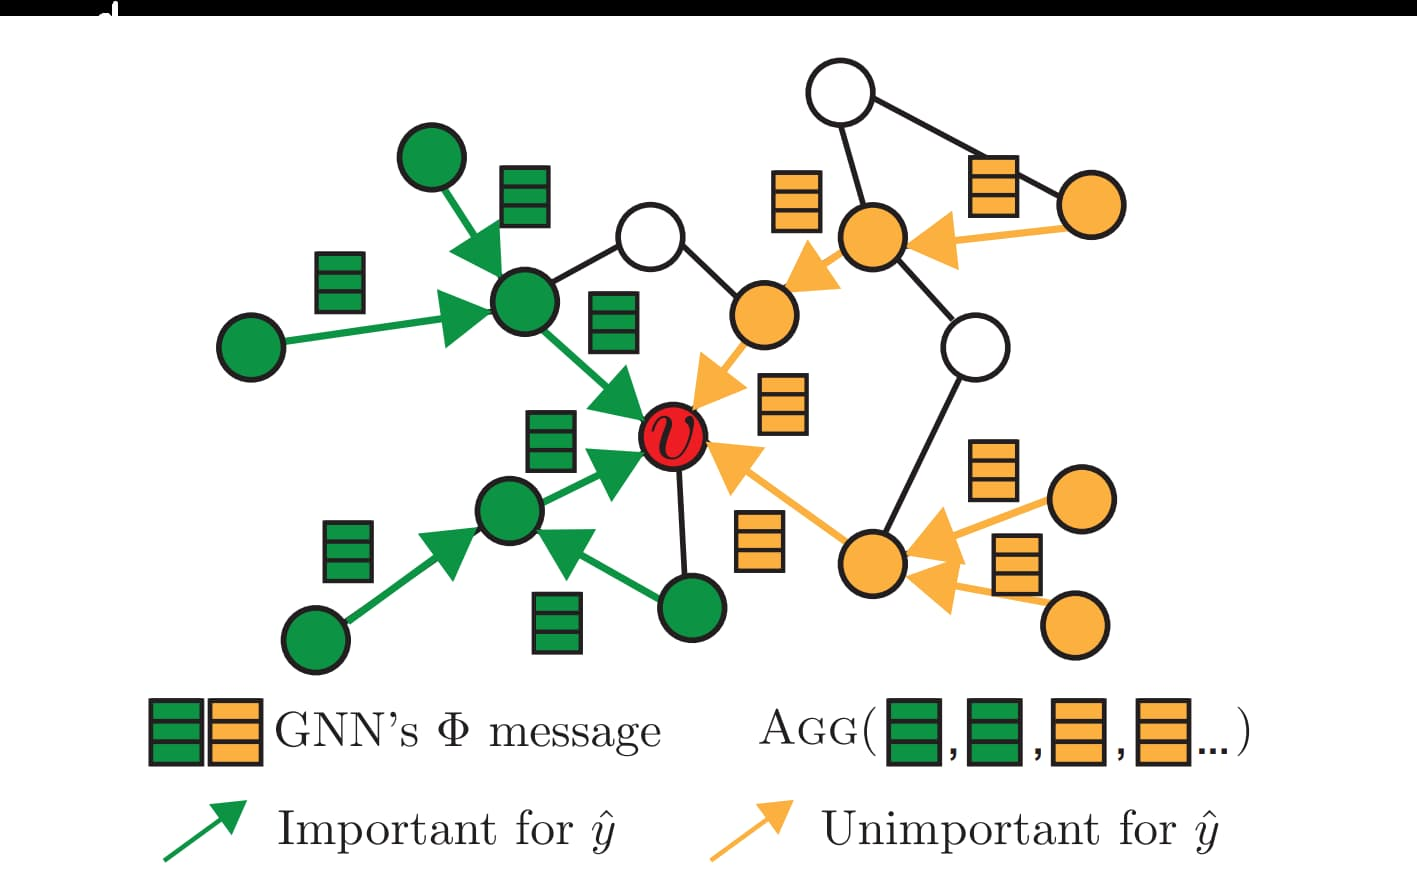
\includegraphics[width=\textwidth]{src/images/chapter2/gnn-explainer.jpg}
    \caption[Ví dụ về một giải thích của GNNExplainer cho một nút]{Ví dụ về việc GNNExplainer đưa ra giải thích ra cho nút $v$ (các nút và cạnh màu xanh là những thành phần quan trọng trong quyết định)}
    \label{fig:gnn_explainer}
\end{figure}

\bigbreak\noindent
Mục tiêu của GNNExplainer khi giải thích cho một dự đoán về một nút trong đồ thị là tìm ra được một đồ thị con chứa các nút và cạnh quan trọng. Từ đó xác định thuộc tính quan trọng trên các nút và mức độ quan trọng của mỗi cạnh của đồ thị con cho dự đoán. Cụ thể, ta có một mô hình $f$ và cần đưa ra giải thích về dự đoán cho nút $x$, $G_S$ là đồ thị con cần tìm từ đồ thị đầu vào $G$ và bộ các thuộc tính của các nút trong $G_S$ (ký hiệu là $X_S$) có ảnh hưởng lớn đến đến quyết định của mô hình. Để xác định được $G_S$ and $X_S$, GNNExplainer thực hiện tối đa hóa thông lượng thông tin tương hỗ (mutual information) $MI$ giữa dự đoán $f(x)$ khi thực hiện trên đồ thị đầu vào $G$ và dự đoán $f(x)$ khi thực hiện trên đồ thị $G_S$ với tập thuộc tính $X_S$ như công thức sau:

\begin{equation} \label{eq:chapter2_gnnexplainer_mi}
    \max_{G_S}MI(Y,(G_S, X_S)) = H(Y) - H(Y|G=G_S,X=X_S)
\end{equation}

\bigbreak\noindent
Trong đó, $H$ là hàm tính toán entropy với hàm tính phân phối xác xuất $f$, $H(Y|G=G_S,X=X_S)$ là entropy của dự đoán $Y$ được tạo bởi $f$ và $x$ trong trường hợp đồ thị $G_S$ với tập thuộc tính $X_S$, và $H(Y)$ entropy của dự đoán $Y$ được tạo bởi $f$ và $x$ trong trường hợp đồ thị $G$. Ngoài ra ta có công thức của entropy có điều kiện $H(Y|G=G_S,X=X_S)$ biểu diễn trong \textbf{Công thức \ref{eq:chapter2_gnnexplainer_conditional}}:

\begin{equation} \label{eq:chapter2_gnnexplainer_conditional}
    H(Y|G=G_S,X=X_S) = -E_{Y|G_S,X_S} [log P_f(Y |G=G_S,X=X_S)] 
\end{equation}

\bigbreak\noindent
Do $x$ và $f$ luôn cố định nên việc ta cần làm là tối thiểu entropy có điều kiện $H(Y|G=G_S,X=X_S)$, chúng ta sẽ thu được đồ thị con $G_s$ với các cạnh và các thuộc tính của các nút có ảnh hưởng lớn đến quyết định của mô hình.

\bigbreak\noindent
Từ ý tưởng ban đầu trên, GNNExplainer đã được phát triển nhằm có khả năng giải thích cho các công việc khác nhau của GNN như dự đoán cạnh và dự đoán đồ thị. Ngoài ra, GNNExplainer có thể giải thích cho nhiều kiến trúc GNN khác nhau mà không cần phải thay đổi cấu trúc của mô hình GNN.

\subsection{Ý nghĩa của học máy khả giải đối với các hệ thống bảo mật}

Ngày càng nhiều hệ thống bảo mật được tích hợp các mô hình AI nhằm phát hiện các cuộc tấn công mới. Học máy khả giải giúp cung cấp giải thích cho quyết định của hệ thống, giúp người quản trị và nhà nghiên cứu hiểu rõ hơn về lý do tại sao một quyết định cụ thể đã được đưa ra. Học máy khả giải cũng có thể giúp xác định các lỗ hổng trong mô hình học máy của hệ thống bảo mật, từ đó cải thiện tính an toàn và độ tin cậy của hệ thống, tránh việc bị qua mặt bởi các mối đe doạ. Ngoài ra, một hệ thống bảo mật mà người dùng không tin tưởng và không chấp nhận là vô ích. Học máy khả giải có thể giúp xây dựng niềm tin và chấp nhận từ phía người dùng bằng cách giải thích quyết định một cách minh bạch và dễ hiểu. Hiện nay, đã có nhiều nghiên cứu học máy khả giải trong cách lĩnh vực bảo mật như pháp chứng kỹ thuật số, IDS, phát hiện mã độc, phát hiện thư rác và lừa đảo, phát hiện botnet, ... 

\section{Mạng SDN}

\subsection{Tổng quan}

Các hệ thống mạng truyền thống, sử dụng các switch, router cùng với các thiết bị mạng vật lý, cùng với đó là việc cấu hình mạng tại chính thiết bị vật lý gây mất thời gian, dễ gây lỗi và khó gỡ lỗi. Ngoài ra, phần cứng trở nên thiếu linh hoạt vì phụ thuộc vào nhà cung cấp, các phần mềm giao thức độc quyền, mang lại rất nhiều điều bất cập trong quản lý hạ tầng mạng cũng như là chi phí vận hành bảo dưỡng. Theo đó, mạng SDN được ra đời nhằm quản lý hệ, cấu hình, theo dõi hệ thống mạng một cách linh hoạt. Từ đó, cải thiện hiệu suất cũng như khả năng mở rộng của hệ thống mạng.

\bigbreak\noindent
SDN là một hướng đi đầy tiềm năng khi hầu hết tất cả các thiết bị mạng đều có thể được ảo hoá, mang lại sự tự do trong cài đặt, cho phép sử dụng kết hợp nhiều loại thiết bị ảo hoá (kể cả mã nguồn mở), tiết kiệm chi phí, giúp tạo một trường phù hợp với tất cả các phần cứng mà không gây ảnh hưởng đến nhau. Hơn thế nữa, việc ảo hóa thiết bị mạng cung cấp khả năng quản lý một cách tập trung tất cả các thiết bị trong hệ thống mạng, từ có có thể cấu hình một cách hiệu quả và tăng khả năng mở rộng cho hệ thống mạng.

\subsection{Kiến trúc}

\begin{figure}[ht]
    \centering
    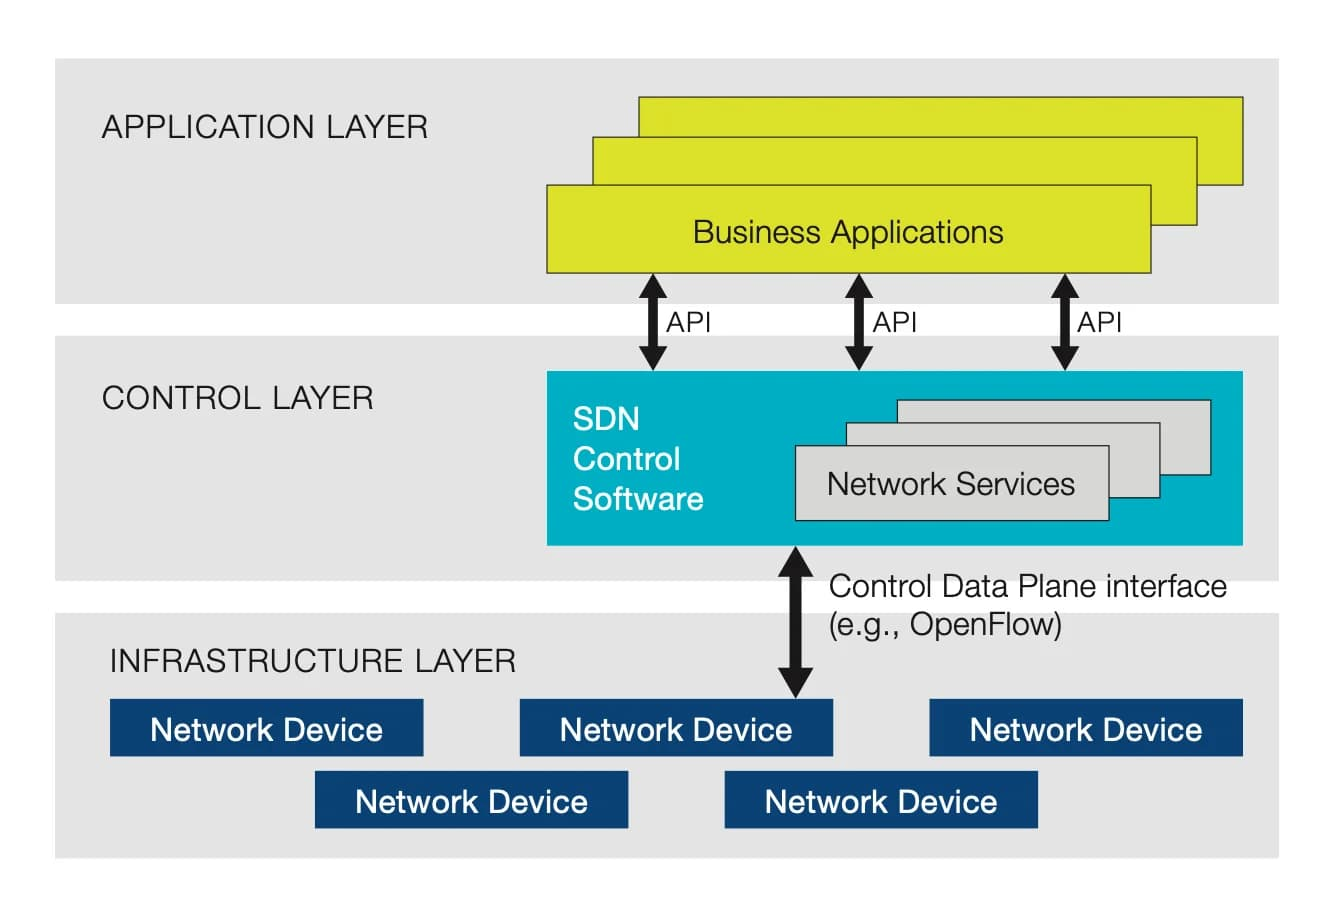
\includegraphics[width=\textwidth]{src/images/chapter2/sdn.jpg}
    \caption{Kiến trúc tổng quan của mạng SDN}
    \label{fig:sdn}
\end{figure}

\bigbreak\noindent
SDN ánh xạ hệ thống mạng theo lớp, cho phép các lớp giao tiếp với nhau thông qua các API. Từ đó các lớp không cần phải giao tiếp vật lý với trung tâm điều khiển. Cụ thể SDN bao gồm ba lớp như sau: lớp điều khiển, lớp hạ tầng và lớp ứng dụng như mô tả trong \textbf{Hình \ref{fig:sdn}}.

\begin{itemize}
    \item \textit{Lớp điều khiển}: Bao gồm một trung tâm điều khiển, nhằm vận hành mọi hoạt động của SDN. Trung tâm điều khiển quản lý các luồng dữ liệu, định tuyến, chuyển tiếp hoặc loại bỏ các gói tin. Lớp điều khiển và lớp hạ tầng giao tiếp với nhau bằng các giao thức như Openflow, NetConf, ..
    \item \textit{Lớp hạ tầng}: Bao gồm các thiết bị mạng như router, switch và các điểm truy cập. Switch có thể tồn tại ở cả dạng ảo như Open vSwitch, Indigo, Pica8,.. và dạng vật lý. Mục đích chính của tầng này là trung chuyển các gói tin theo các quy tắc đã được cấu hình.
    \item \textit{Lớp ứng dụng}: Lớp này đảm nhận việc chạy các ứng dụng như các ứng dụng liên quan đến hoạt động của tổ chức, các ứng dụng như IDS, IPS, tường lửa, .... Lớp này giao tiếp với lớp điều khiển bằng giao thức A-CPI (Application Control Plane Interface).
\end{itemize}

\subsection{Tiềm năng của mạng SDN trong việc chống lại tấn công APT}

Bộ điều khiển SDN cung cấp cái nhìn tổng thể về toàn bộ hệ thống mạng. Với khả năng này, bộ điều khiển SDN có thể hỗ trở cho nhiều giải pháp bảo mật và trở thành phương tiện thực tiễn trong triển khai các giải pháp phát hiện tấn công APT. Trên thực tế, các ứng dụng tiềm năng của SDN trong các giải pháp bảo mật đã được chứng minh bởi \cite{farris2018survey}, \cite{yurekten2021sdn}, \cite{zarca2020virtual}. Ngoài ra, đã có nhiều nghiên cứu \cite{abdel2021federated}, \cite{thi2022federated}, \cite{mothukuri2021federated} thành công trong việc tận dụng khía cạnh này của SDN kết hợp với các phương pháp học liên kết để phát hiện các cuộc tấn công mạng.
